\documentclass[conference, onecolumn]{IEEEtran}
\IEEEoverridecommandlockouts
\usepackage{cite}
\usepackage{amsmath,amssymb,amsfonts}
\usepackage{algorithmic}
\usepackage{graphicx}
\usepackage{textcomp}
\usepackage{xcolor}
\usepackage{flushend}
\usepackage{hyperref}
\usepackage{adjustbox}
\usepackage{float}
\usepackage{booktabs}
\usepackage{array}
\usepackage[utf8]{inputenc}
\usepackage[T5]{fontenc}  % Hoặc T1 nếu bạn không cần tiếng Việt
%\usepackage[vietnamese]{babel}
%%%%%%%%%%%%%%%%%%%%%
\usepackage{tikz}
\usetikzlibrary{shapes.geometric, arrows.meta, positioning}
\usepackage[utf8]{inputenc}   % Nếu file .tex có Unicode
\usepackage[T1]{fontenc}      % Để xử lý tiếng Việt, dấu
\usepackage[english]{babel}   
\usepackage{fancyhdr}
%%%%%%%%%%%%%%%%%%%%%
\def\BibTeX{{\rm B\kern-.05em{\sc i\kern-.025em b}\kern-.08em
    T\kern-.1667em\lower.7ex\hbox{E}\kern-.125emX}}
\begin{document}

\title{Smart Door Lock\\
{\large IOT102-SE1815, Group 2}}
\pagestyle{fancy}
\fancyhf{} 
\renewcommand{\headrulewidth}{0pt}
\fancyfoot[C]{\thepage}  % Số trang ở giữa footer
\author{
Le Pham Hoai Bao, Vu Minh Quang, Nguyen Minh Thanh, Hoang Bao Thach, and Le The Dung\\
FPT University, Ho Chi Minh Campus, Vietnam\\
\{hoaibaole.qng, vminhquang05, minhthanh2012005, thach2548\}@gmail.com, dunglt96@fe.edu.vn}
\maketitle

\begin{abstract}
This project presents the comprehensive design and implementation of a multi-modal smart door lock system aimed at enhancing residential security and improving user convenience. The system is built around an Arduino Uno microcontroller, which functions as the central processing unit responsible for handling input signals, executing authentication logic, and controlling output devices. Multiple hardware components are integrated to provide a layered access control mechanism. These include an ultrasonic sensor (HC-SR04) for detecting human presence near the entry point, which triggers the activation of the system; a 4x4 matrix keypad for secure PIN-based authentication; an RC522 RFID reader module that supports contactless access via MIFARE-compatible cards or key fobs; and an HC-05 Bluetooth module, allowing authorized users to unlock the door remotely through a custom-built smartphone application.
To further expand the system’s capabilities, a NodeMCU ESP8266 module is employed to provide Wi-Fi connectivity, enabling real-time data transmission to the ThingSpeak IoT cloud platform. This integration allows users to remotely monitor system status, receive alerts, and log access events for enhanced situational awareness and auditability. The electromagnetic lock mechanism is controlled via a relay module, which is triggered upon successful authentication by any of the supported input methods.
The system supports three primary modes of entry: PIN input via keypad, RFID card scanning, and Bluetooth-based commands from a paired smartphone. This redundancy improves both usability and fault tolerance. The software architecture leverages modular coding practices and utilizes open-source libraries such as \texttt{Keypad.h}, \texttt{MFRC522.h}, and \texttt{SoftwareSerial.h}, ensuring ease of development and maintainability.
Experimental validation was conducted under typical residential operating conditions. Results indicate that the system performs reliably across all authentication methods, with response times averaging under one second. The integration of local and wireless communication channels ensures a robust and flexible platform that satisfies essential security requirements. Furthermore, the modular hardware and software design provide a scalable foundation for future upgrades, such as biometric integration, two-factor authentication, or cloud-based user management. Overall, the system demonstrates an effective balance between functionality, security, and ease of use, making it a practical solution for modern smart home applications.
\end{abstract}

\section{Introduction}
With the continued acceleration of global urbanization and the increasing integration of technology into daily life, the demand for secure, automated, and convenient access control systems has grown substantially. Residential and commercial environments alike are facing evolving challenges in terms of physical security. Traditional mechanical locking systems—although long-standing—are increasingly inadequate in preventing unauthorized access. Their vulnerabilities include key duplication, lock picking, and brute-force break-ins, which have been documented as common intrusion methods in urban environments [1].

These threats are compounded by modern lifestyle demands for mobility, flexibility, and remote control. For instance, tenants may wish to grant temporary access to guests, delivery services, or maintenance personnel without physically handing over a key. The inability of traditional locks to adapt to such use cases has accelerated interest in "smart locks"—advanced systems that combine sensing, wireless communication, and programmable control mechanisms [2].

Smart door lock systems signify a paradigm shift in access control technology. These systems utilize embedded electronics and microcontroller platforms to implement digital access methods such as PIN codes, RFID scanning, smartphone-based authentication, or biometric input. Through wireless modules such as Bluetooth, Wi-Fi, or GSM, they can be remotely operated and monitored, offering real-time updates on access logs and door status. By integrating with home automation platforms, smart locks can also participate in broader IoT ecosystems for energy efficiency and safety [2], [5].

This project proposes the development of a smart door locking system that uses a combination of proximity sensing, RFID identification, Bluetooth communication, and password verification. The hardware architecture centers around the Arduino Uno microcontroller, selected for its cost-effectiveness, open-source community support, and versatility in handling sensor inputs and actuator outputs [3]. Several peripheral modules are incorporated:

The proposed smart door locking system integrates several key components that collectively enable multi-factor authentication and intelligent access control. At the heart of the system is the Arduino Uno microcontroller, which coordinates data from all sensors and executes decision logic. To detect the presence of a person near the entrance, the HC-SR04 ultrasonic sensor is employed; it measures the distance to nearby objects using high-frequency sound waves, allowing the system to remain in a low-power or standby state until someone approaches. For identity verification, an MFRC522 RFID reader is used to scan contactless RFID cards, which carry unique identifiers pre-registered in the system's memory. Complementing this, a 4x4 matrix keypad is available for users to input a numeric password, providing an additional layer of security through knowledge-based authentication. Wireless control is achieved through the HC-05 Bluetooth module, which enables communication with a paired smartphone—users can unlock the system via a mobile application or a Bluetooth terminal, offering convenience and flexibility. Once authentication is successful through any combination of these methods, a relay module is triggered to control a magnetic lock, either securing or releasing the door accordingly. This seamless integration of hardware ensures a reliable and scalable access system that supports both physical and digital modes of entry, effectively enhancing residential security in a modern, user-friendly manner.

This system implements multi-factor authentication (MFA), which is highly recommended for modern security solutions [4]. Rather than relying on a single input mode, users can be required to authenticate through a combination of password, card, and proximity checks, or optionally via a trusted smartphone. This layered security model significantly increases system robustness and reduces the risk posed by the compromise of any individual access method.

The relevance of this project extends beyond practical application. It also functions as an educational framework that introduces students, hobbyists, and engineers to key concepts in embedded systems, digital electronics, and wireless communication. Each component used in this system (e.g., RFID, Bluetooth, ultrasonic sensors) has standalone learning value and can be independently extended in future versions.

Furthermore, the modularity of the system opens the door to scalability and enhancement. For example, future iterations may integrate a fingerprint sensor, a camera module for facial recognition, or even IoT cloud-based control via platforms like Blynk or Firebase. These improvements can transform the current offline prototype into a fully networked and intelligent door control platform [5].

In conclusion, this smart door lock project addresses both the increasing societal need for adaptable home security solutions and the educational opportunity to explore real-world embedded applications. It demonstrates how low-cost hardware, when thoughtfully integrated, can provide meaningful functionality and set the stage for more sophisticated future developments.

\begin{figure*}[htb]
	\centering
	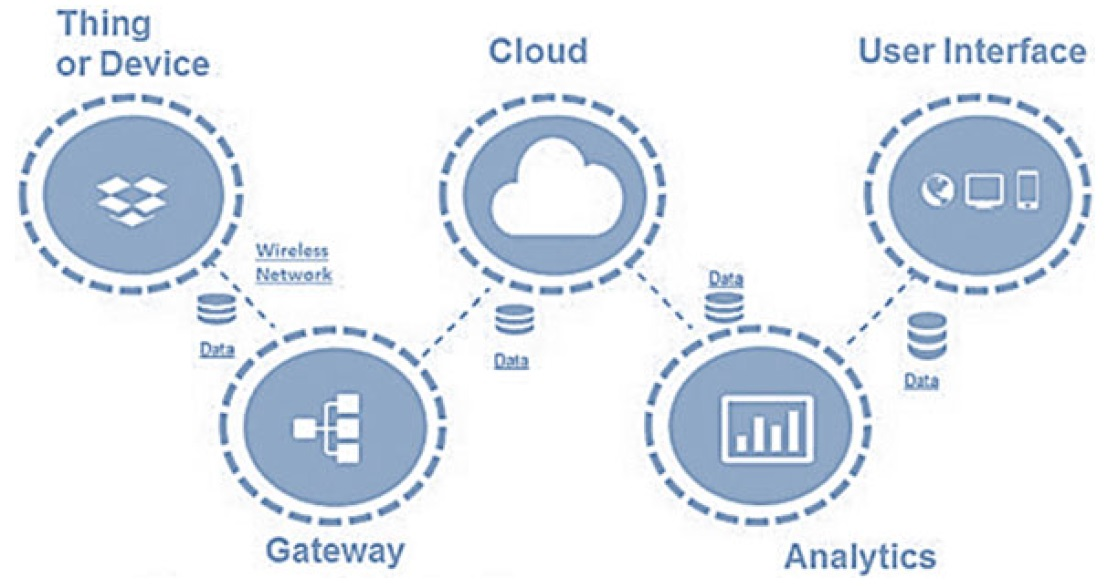
\includegraphics[width=0.4\textwidth]{IoT_Components.jpg}
	\caption{Major components of IoT system.}
	\label{fig1}
\end{figure*}

\section{Methods and Materials}

\subsection{System Model and Block Diagram}

\begin{figure}[H]
	\centering
	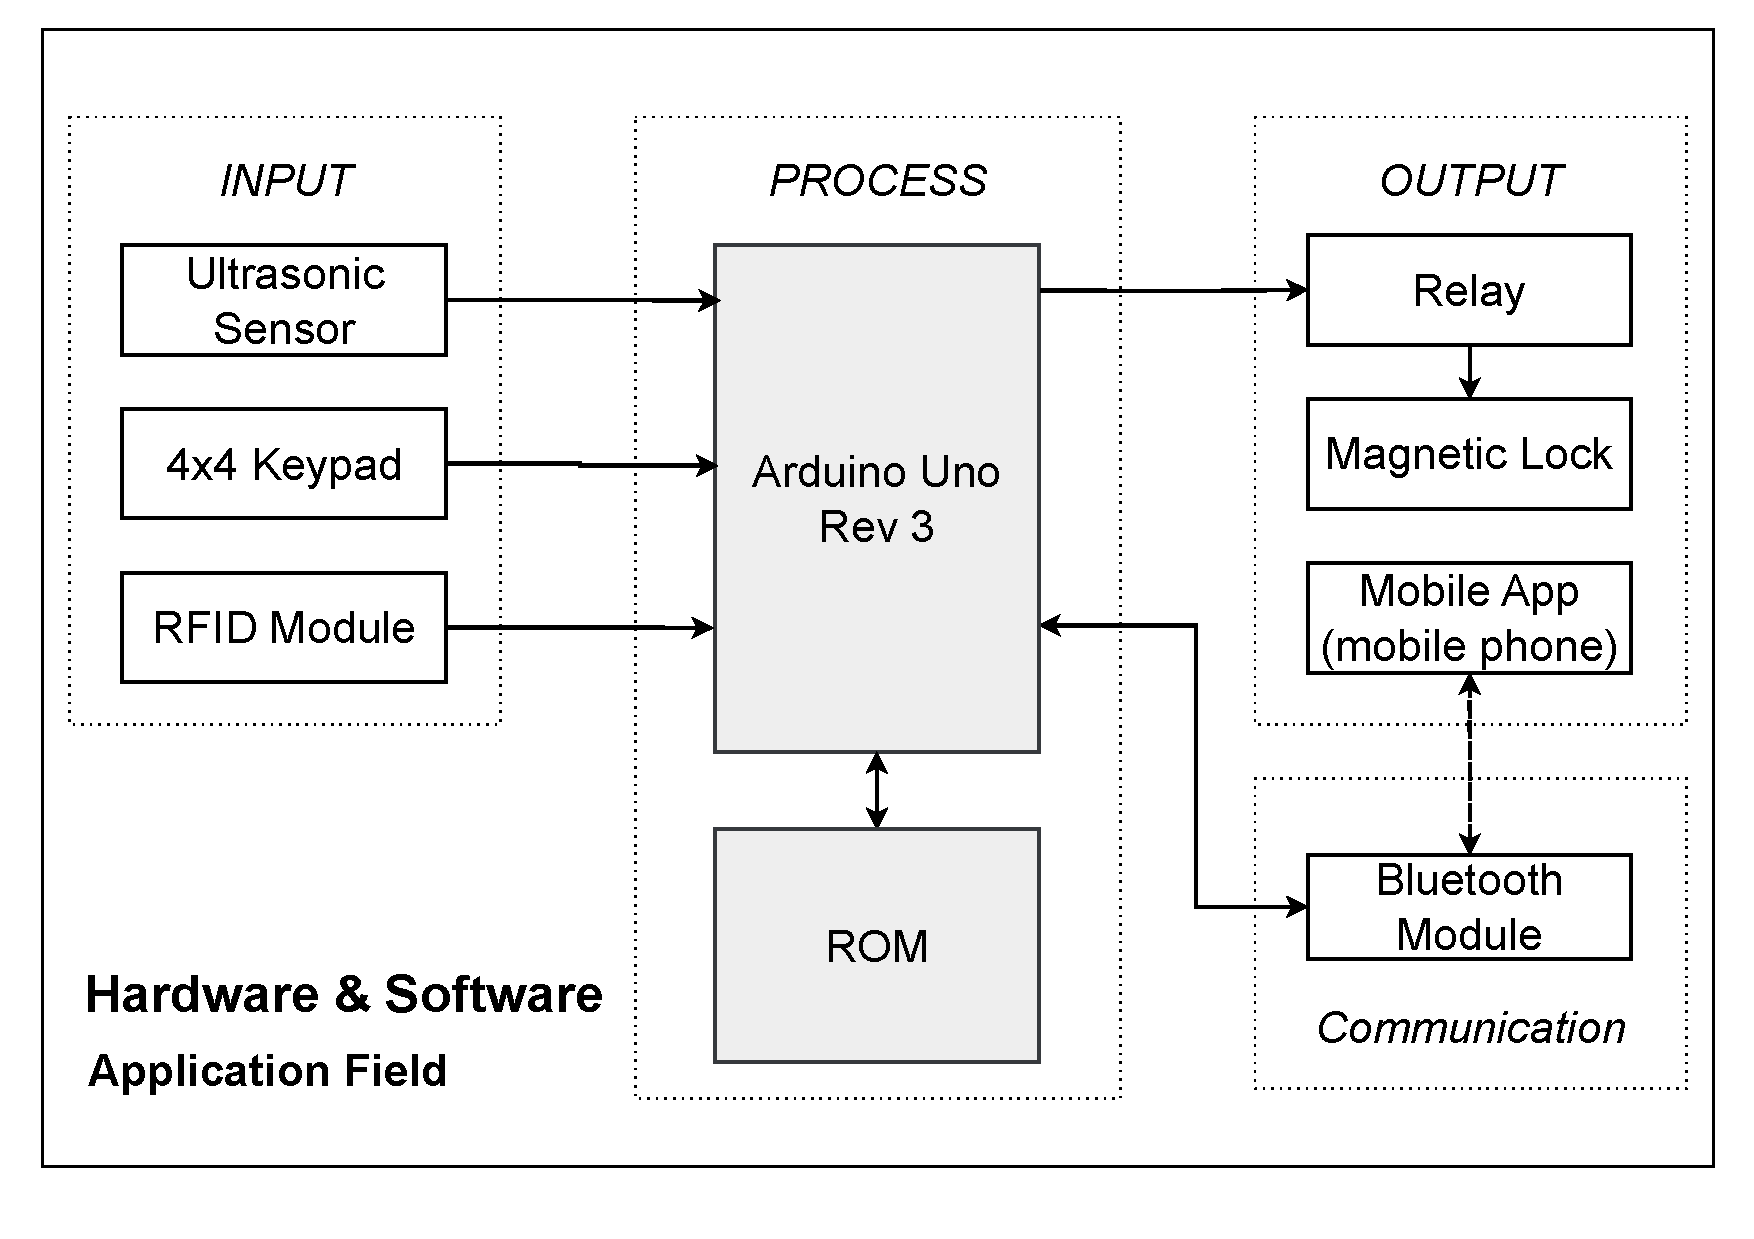
\includegraphics[width=0.55\textwidth]{blockdia (1).pdf}
	\caption{Block diagram of the proposed system.}
	\label{fig2}
\end{figure}
The smart door lock system is structured into four functional blocks: input, processing, output, and communication. The input block comprises an ultrasonic distance sensor (HC-SR04), a 4x4 membrane keypad, and an RFID reader module (MFRC522), each responsible for capturing real-world signals related to user interaction and presence. The ultrasonic sensor continuously monitors the area near the door to detect human presence within a predefined range (typically under 100~cm), serving as a trigger for activating the rest of the system. Once presence is detected, the Arduino initiates the authentication sequence by enabling keypad and RFID scanning. The keypad allows users to manually input a personal identification number (PIN), while the RFID module scans contactless cards or key tags and transmits the unique identifier to the microcontroller via SPI communication. The processing block is centered around the Arduino Uno Rev3, which acts as the core controller. It evaluates incoming input signals in real-time and compares them against stored credentials (predefined RFID UIDs and PINs) located in the microcontroller’s flash memory or EEPROM. Conditional logic is used to determine whether the input data matches authorized entries. If access is granted, the Arduino activates the output block, which consists primarily of a relay module that switches 12~V power to the electromagnetic lock. This causes the door to unlock temporarily, after which a timed re-locking mechanism is automatically engaged to restore security. Simultaneously, user feedback (e.g., LED indicators or optional buzzers) can be triggered to signal successful or failed authentication attempts. The communication block is managed by the HC-05 Bluetooth module, which enables serial wireless communication with a paired smartphone. This allows the system to receive remote unlock commands or send real-time status updates to a mobile application. The communication layer complements local authentication by offering an additional interface for user control and monitoring, making the system suitable for both residential and office environments where convenience and security are equally prioritized. Overall, the modular block-based architecture ensures maintainability, scalability, and future extensibility—allowing easy integration of components such as fingerprint scanners, network-based logging, or camera modules in future upgrades.

\subsection{Components and Peripheral Devices}
	 \textbf{Arduino Uno:} The Arduino Uno R3 is a widely adopted microcontroller board based on the ATmega328P. It is commonly used as the central processing unit in Internet of Things (IoT) applications due to its ease of use and robust hardware features. The board provides 14 digital input/output (I/O) pins (D0–D13), six of which (D3, D5, D6, D9, D10, D11) support pulse-width modulation (PWM) for analog signal control.
	Pins D0 (RX) and D1 (TX) are reserved for UART communication and are typically avoided in projects involving Bluetooth modules to prevent conflicts. Digital pins D10–D13 support the Serial Peripheral Interface (SPI) protocol, while six analog input pins (A0–A5) facilitate interfacing with analog sensors. Power interfaces include regulated 5V and 3.3V outputs, ground (GND), and a VIN pin for supplying external voltages in the 7–12 V range.
	The board is programmed using the Arduino Integrated Development Environment (IDE), which features a simplified syntax and extensive library support, making it suitable for both beginners and professionals.
	
	\begin{figure}[H]
		\centering
		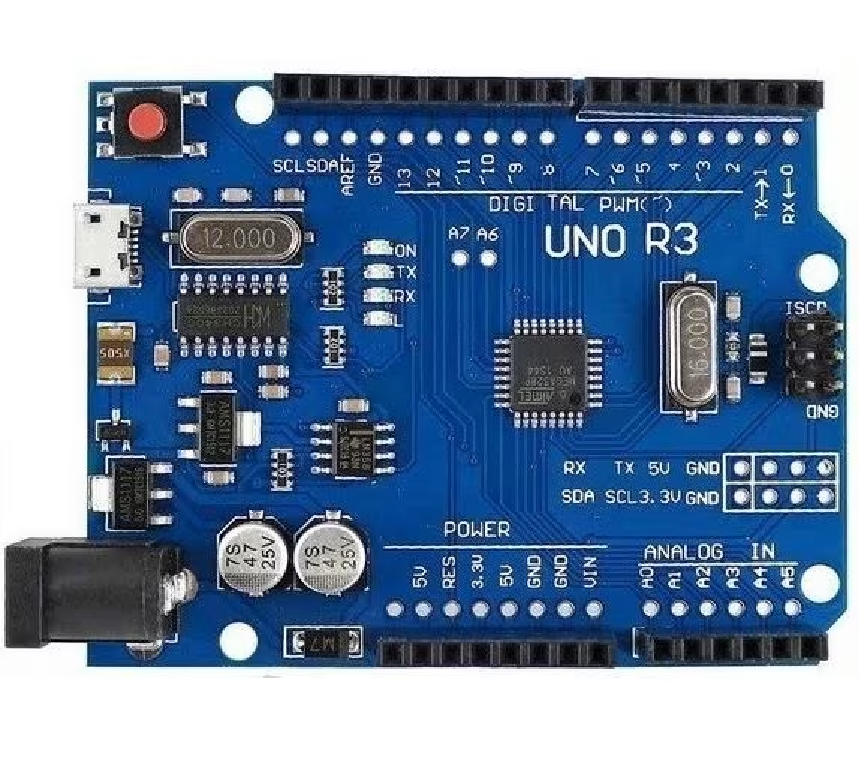
\includegraphics[width=0.5\textwidth]{UNOR3.pdf}
		\caption{Arduino Uno R3 microcontroller board.}
		\label{fig3}
	\end{figure}

%-------%
 \textbf{HC-05:} The HC-05 is a widely adopted Bluetooth SPP (Serial Port Protocol) module specifically designed for wireless serial communication in embedded systems. It enables seamless interaction between microcontrollers—such as the Arduino Uno—and Bluetooth-enabled devices including smartphones, tablets, and laptops. One of the key advantages of the HC-05 is its ability to operate in both Master and Slave modes, making it highly adaptable for a wide range of Internet of Things (IoT) and automation applications. The module communicates through UART using TX and RX pins, and it typically runs at a default baud rate of 9600 bps, though this can be customized using AT commands. These commands also allow users to modify various settings, such as the module name, pairing password, operating mode, and data rate, which adds flexibility when integrating it into more complex systems.
 The HC-05 operates on the Bluetooth 2.0 + EDR (Enhanced Data Rate) standard, offering a stable wireless range of up to 10 meters in open environments, which is sufficient for most home automation scenarios. Although the Bluetooth chip inside the module functions at 3.3V, the board is usually equipped with an onboard voltage regulator and logic level shifter, allowing safe interfacing with 5V microcontrollers like the Arduino Uno. This hardware compatibility makes it easier to incorporate the HC-05 into beginner and advanced projects alike, without requiring additional components for voltage conversion.
 In the context of the proposed smart door lock system, the HC-05 plays a crucial role in providing wireless access control. It enables authorized users to connect to the system via their smartphones and send unlock commands remotely. This functionality significantly enhances user convenience, especially in scenarios where users may not have immediate access to a keypad or RFID card. Moreover, unlike Wi-Fi or internet-dependent solutions, the Bluetooth-based setup does not rely on network infrastructure, making it more resilient in areas with limited connectivity. The low power consumption, ease of configuration, and reliable data transmission make the HC-05 an ideal choice for enhancing both security and usability in smart access control systems.
 
\begin{figure}[H]
	\centering
	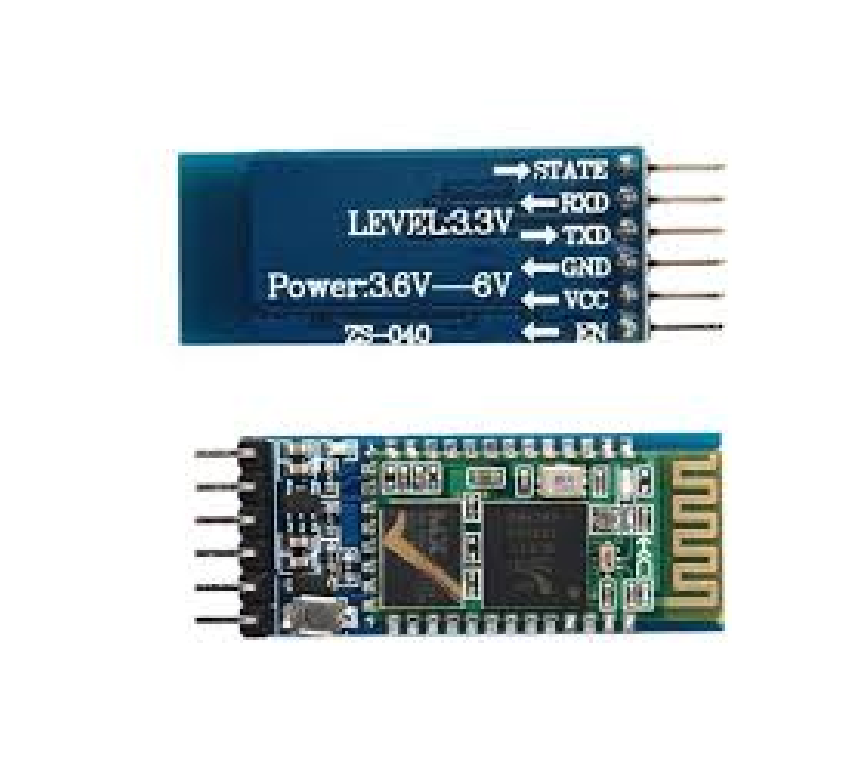
\includegraphics[width=0.65\textwidth]{HC_05.pdf}
	\caption{HC-05 Bluetooth module.}
	\label{fig}
\end{figure}
	
 \textbf{Ultrasonic Sensor (HC-SR04):} The HC-SR04 ultrasonic sensor is a widely used non-contact distance measurement device in embedded and smart automation systems. It operates by emitting a high-frequency ultrasonic pulse via the TRIG pin and measuring the time it takes for the echo to return to the ECHO pin after bouncing off an object. The sensor has four pins: VCC for power input, GND for ground, TRIG for sending the trigger signal, and ECHO for receiving the reflected signal. It supports a distance range from approximately two centimeters up to four meters with a typical accuracy of around three millimeters and is fully compatible with five-volt digital logic, making it suitable for microcontrollers like the Arduino Uno. In the proposed smart door lock system, the HC-SR04 is used to detect the presence of a person within a defined range, typically less than half a meter. Upon detection, the system automatically shifts from standby to active mode, enabling other authentication subsystems such as keypad input, RFID scanning, or Bluetooth communication. The sensor is controlled through straightforward digital input and output operations using Arduino functions like digitalWrite and pulseIn, requiring no additional libraries. For best performance, it should be installed facing the approach direction of the user with minimal physical obstructions. Hard, flat surfaces enhance signal accuracy, while soft, irregular, or angled objects may result in less reliable measurements. Additionally, external ultrasonic noise sources should be avoided to prevent interference. Due to its simplicity, low cost, and reliability, the HC-SR04 remains a highly effective solution for proximity detection in smart door access and other automation applications.

\begin{figure}[H]
	\centering
	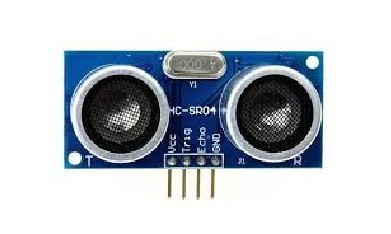
\includegraphics[width=0.6\textwidth]{Ultrasonic_sensor.pdf}
	\caption{HC-SR04 ultrasonic sensor.}
	\label{fig4}
\end{figure}

 \textbf{4x4 Keypad:} The 4×4 matrix keypad is a widely used input device comprising 16 tactile push buttons arranged in a matrix of four rows (R1–R4) and four columns (C1–C4), enabling numeric or alphanumeric input. It operates at 5~V DC and communicates through digital I/O, requiring eight interface pins. The device functions based on matrix scanning, where pressing a key connects a unique pair of row and column lines. The microcontroller sequentially activates column signals while monitoring the row lines to detect the key press, which reduces the number of required I/O pins compared to discrete button wiring. In the proposed smart door lock system, the keypad serves as a primary user interface for entering a personal identification number (PIN) during authentication. It is connected to eight digital I/O pins of the Arduino Uno and is periodically scanned to capture user input. For software integration, the Arduino \texttt{Keypad.h} library is commonly employed, offering built-in functions for matrix scanning and software debouncing, and supporting real-time single or multi-key detection. From a design perspective, the keypad should be mechanically secured to prevent false detections due to movement or bounce, and long wiring runs should be avoided to minimize signal interference. Given its low cost, robustness, and ease of implementation, the 4×4 keypad is a practical and reliable solution for secure input in embedded systems, particularly in applications such as electronic locks, access control, and vending machines.

\begin{figure}[H]
	\centering
	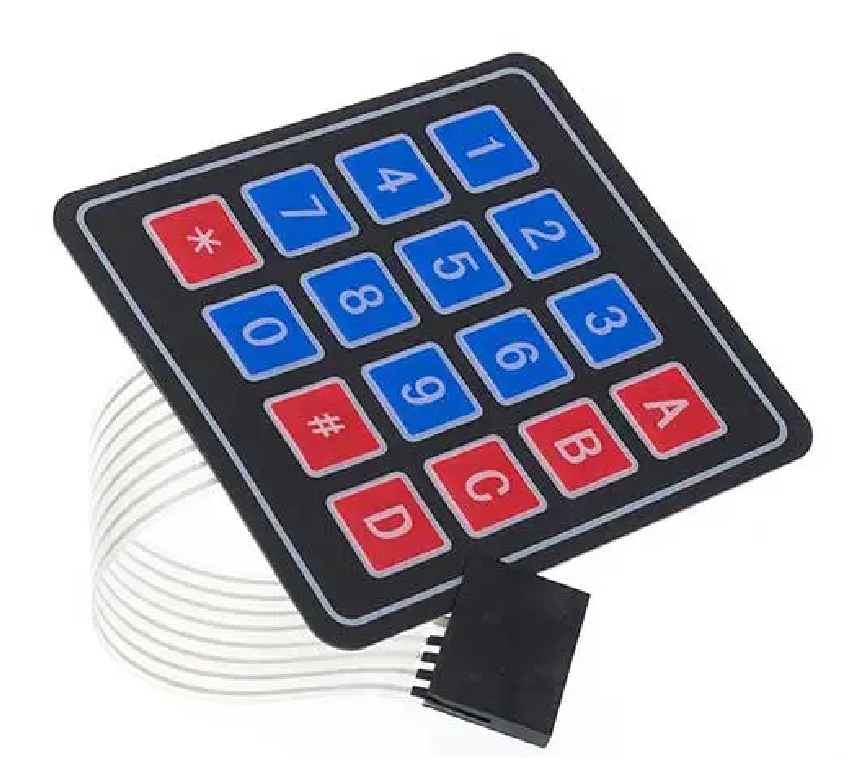
\includegraphics[width=0.4\textwidth]{KEYpad.pdf}
	\caption{4×4 matrix keypad.}
	\label{fig5}
\end{figure}

 \textbf{RFID RC522:} The RC522 is a compact and cost-effective RFID (Radio Frequency Identification) reader module that operates at 13.56~MHz and is compatible with MIFARE standard contactless cards and tags. It is commonly used in access control systems for secure wireless identification through electromagnetic coupling. The module operates at 3.3~V DC and communicates with microcontrollers via the Serial Peripheral Interface (SPI) protocol. It typically supports a reading range of 2–5~cm and includes seven primary pins: SDA (Slave Select), SCK (Serial Clock), MOSI (Master Out Slave In), MISO (Master In Slave Out), RST (Reset), VCC (3.3~V power input), and GND (ground). When a tag enters the module’s range, the RC522 emits an electromagnetic field to energize the passive RFID tag, which then transmits its unique identifier (UID) back to the reader. The module relays this UID to the Arduino Uno via SPI, where it is processed for authentication. In the smart door lock system, the RC522 is used as a key component for identity verification, either as a standalone method or in conjunction with other input mechanisms like a keypad or mobile Bluetooth commands. Software integration is facilitated through the open-source \texttt{MFRC522.h} library, which provides high-level APIs for device initialization, UID reading, and authentication logic. Care must be taken to supply regulated 3.3~V power to the module, as higher voltages (e.g., 5~V) can cause permanent damage. Additionally, proper SPI pin alignment must be ensured according to the microcontroller used (e.g., for Arduino Uno: MOSI = D11, MISO = D12, SCK = D13, SDA = D10), and a decoupling capacitor across the power lines is recommended to enhance stability. Thanks to its low power consumption, small footprint, and straightforward integration, the RC522 remains a dependable choice for RFID-based security and identification applications in embedded systems.

\begin{figure}[H]
	\centering
	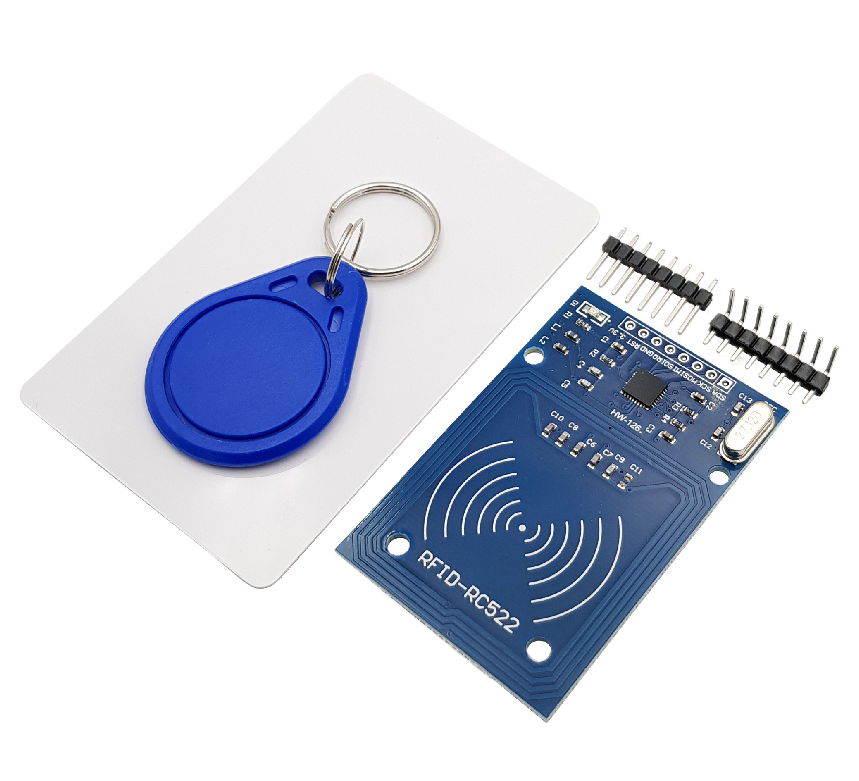
\includegraphics[width=0.5\textwidth]{RFID_RC522.pdf}
	\caption{RC522 RFID reader module.}
	\label{fig6}
\end{figure}

 \textbf{Relay:} A 1-channel relay module is employed in the smart door lock system as an intermediate switching device that allows the Arduino to control high-power electrical components—such as electromagnetic locks, lighting systems, or small appliances—using low-voltage digital outputs. The relay module typically includes three control pins: VCC (5~V power supply), GND (ground), and IN (input control signal), and it operates by magnetically actuating an internal mechanical switch. When the IN pin is driven HIGH or LOW (depending on the module's trigger logic), the relay coil is energized, causing the switch to toggle between the common (COM), normally open (NO), and normally closed (NC) terminals. In this project, the relay is configured in such a way that, upon successful user authentication via keypad, RFID, or Bluetooth, the Arduino sends a control signal to activate the relay, which then connects the 12~V power supply to the magnetic lock, unlocking the door. After a predefined time interval, the Arduino deactivates the relay, re-locking the door automatically. To ensure electrical safety and reliability, most relay modules—including the one used here—feature an integrated opto-isolator (opto-coupler), which electrically isolates the control circuit (Arduino side) from the high-voltage load circuit. This design protects the microcontroller from potential voltage spikes, electromagnetic interference (EMI), or back EMF generated when inductive loads like electromagnetic locks are switched off. Additionally, onboard flyback diodes are typically present across the relay coil to suppress voltage transients, further enhancing operational stability. Overall, the relay module plays a crucial role in bridging the low-power logic of the Arduino with the high-power demands of electromechanical actuators in a safe and efficient manner.

\begin{figure}[H]
	\centering
	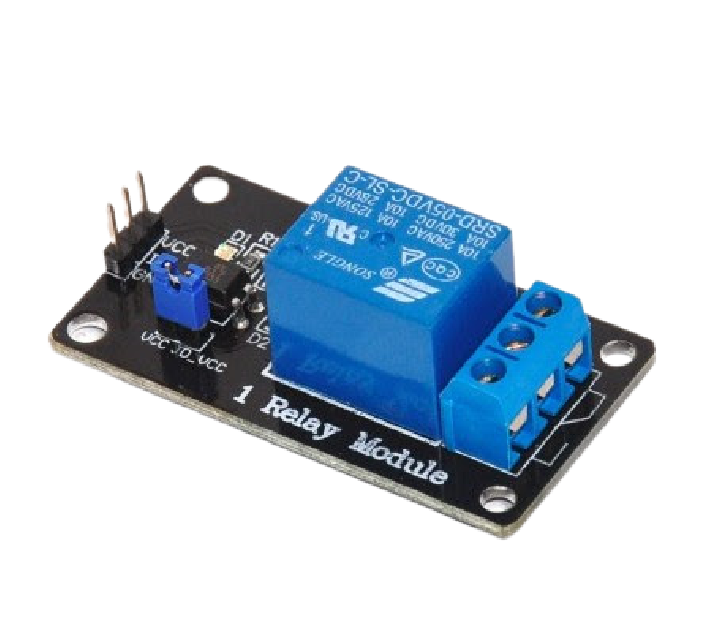
\includegraphics[width=0.4\textwidth]{relay.pdf}
	\caption{Relay.}
	\label{fig7}
\end{figure}	

 \textbf{Magnetic Lock:} The electromagnetic lock used in this system operates at 12~V and functions based on the principle of magnetic attraction generated by electric current. When energized, the lock produces a strong magnetic field that securely binds a metal armature plate to its surface, effectively holding the door closed with a force typically rated between 60--280~kg, depending on the model. As soon as the current is interrupted—either by deactivating the relay through the Arduino or during a power outage—the magnetic field collapses, instantly releasing the door. This behavior classifies it as a \textit{fail-safe} mechanism, meaning it remains locked as long as power is applied and unlocks automatically when power is lost, a feature that aligns with standard fire safety regulations in residential and commercial buildings. In the implemented smart door lock system, the electromagnetic lock draws a relatively high operating current in the range of 0.5--1~A, which can cause voltage instability if not powered independently. Therefore, it is supplied by a dedicated 12~V output from a buck converter sourced directly from a 14.8~V Li-ion battery pack. This separation ensures that the Arduino microcontroller and logic-level peripherals are not affected by fluctuations in the power supply to the lock. Additionally, control of the lock is handled via a relay module with opto-isolation, which allows the low-voltage logic of the Arduino to switch the higher voltage needed for the lock safely and reliably. This configuration enables efficient and robust access control while minimizing risks of electrical interference or microcontroller overload.
 
\begin{figure}[H]
	\centering
	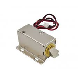
\includegraphics[width=0.35\textwidth]{Magnetic.pdf}
	\caption{Magnetic Lock.}
	\label{fig8}
\end{figure}

\textbf{Circuit Diagram:} The circuit diagram showcases a robust smart door lock system built on the Arduino Uno platform, designed to deliver secure, automated, and user-friendly access control. Acting as the central controller, the Arduino manages various input/output modules to authenticate users, make access decisions, and provide real-time feedback. The system adopts a multi-layered authentication approach for enhanced security and flexibility.
On the input side, it incorporates a 4x4 matrix keypad for PIN code entry, an RFID RC522 module for contactless card authentication, and a Bluetooth HC-05 module that allows smartphones to wirelessly unlock the system. An ultrasonic sensor (HC-SR04) detects human presence within 0.5 meters, activating the system only when necessary, thereby conserving power and enhancing context awareness.
For user feedback, the system uses a buzzer and LED indicators connected to digital pins to provide audio-visual responses. A 16x2 I2C LCD display shows real-time messages like “Access Granted” or “Wrong PIN,” while using minimal wiring and preserving I/O pins.
The relay module plays a critical role in controlling an electromagnetic lock or servo motor, switching it on or off based on successful authentication. Power is supplied by three 18650 lithium-ion batteries connected in series, providing a total of approximately 12.6V when fully charged. This voltage is regulated through a power management module to ensure stable 5V and 3.3V outputs, effectively protecting sensitive components such as the RFID reader and microcontroller from overvoltage damage.
All modules are connected on a solderless breadboard, with organized color-coded wiring for VCC, GND, and data/control lines. This layout ensures easy debugging, modularity, and clear component management—ideal for prototyping and educational use.
In conclusion, the system offers a well-rounded, multi-modal smart access solution, combining PIN, RFID, Bluetooth, and presence detection with intuitive feedback. Its modular design and expandability make it suitable for smart homes and offices, and it can be further enhanced with Wi-Fi modules (e.g., ESP8266) or cloud-based monitoring, aligning with the broader IoT ecosystem.

\begin{figure}[H]
	\centering
	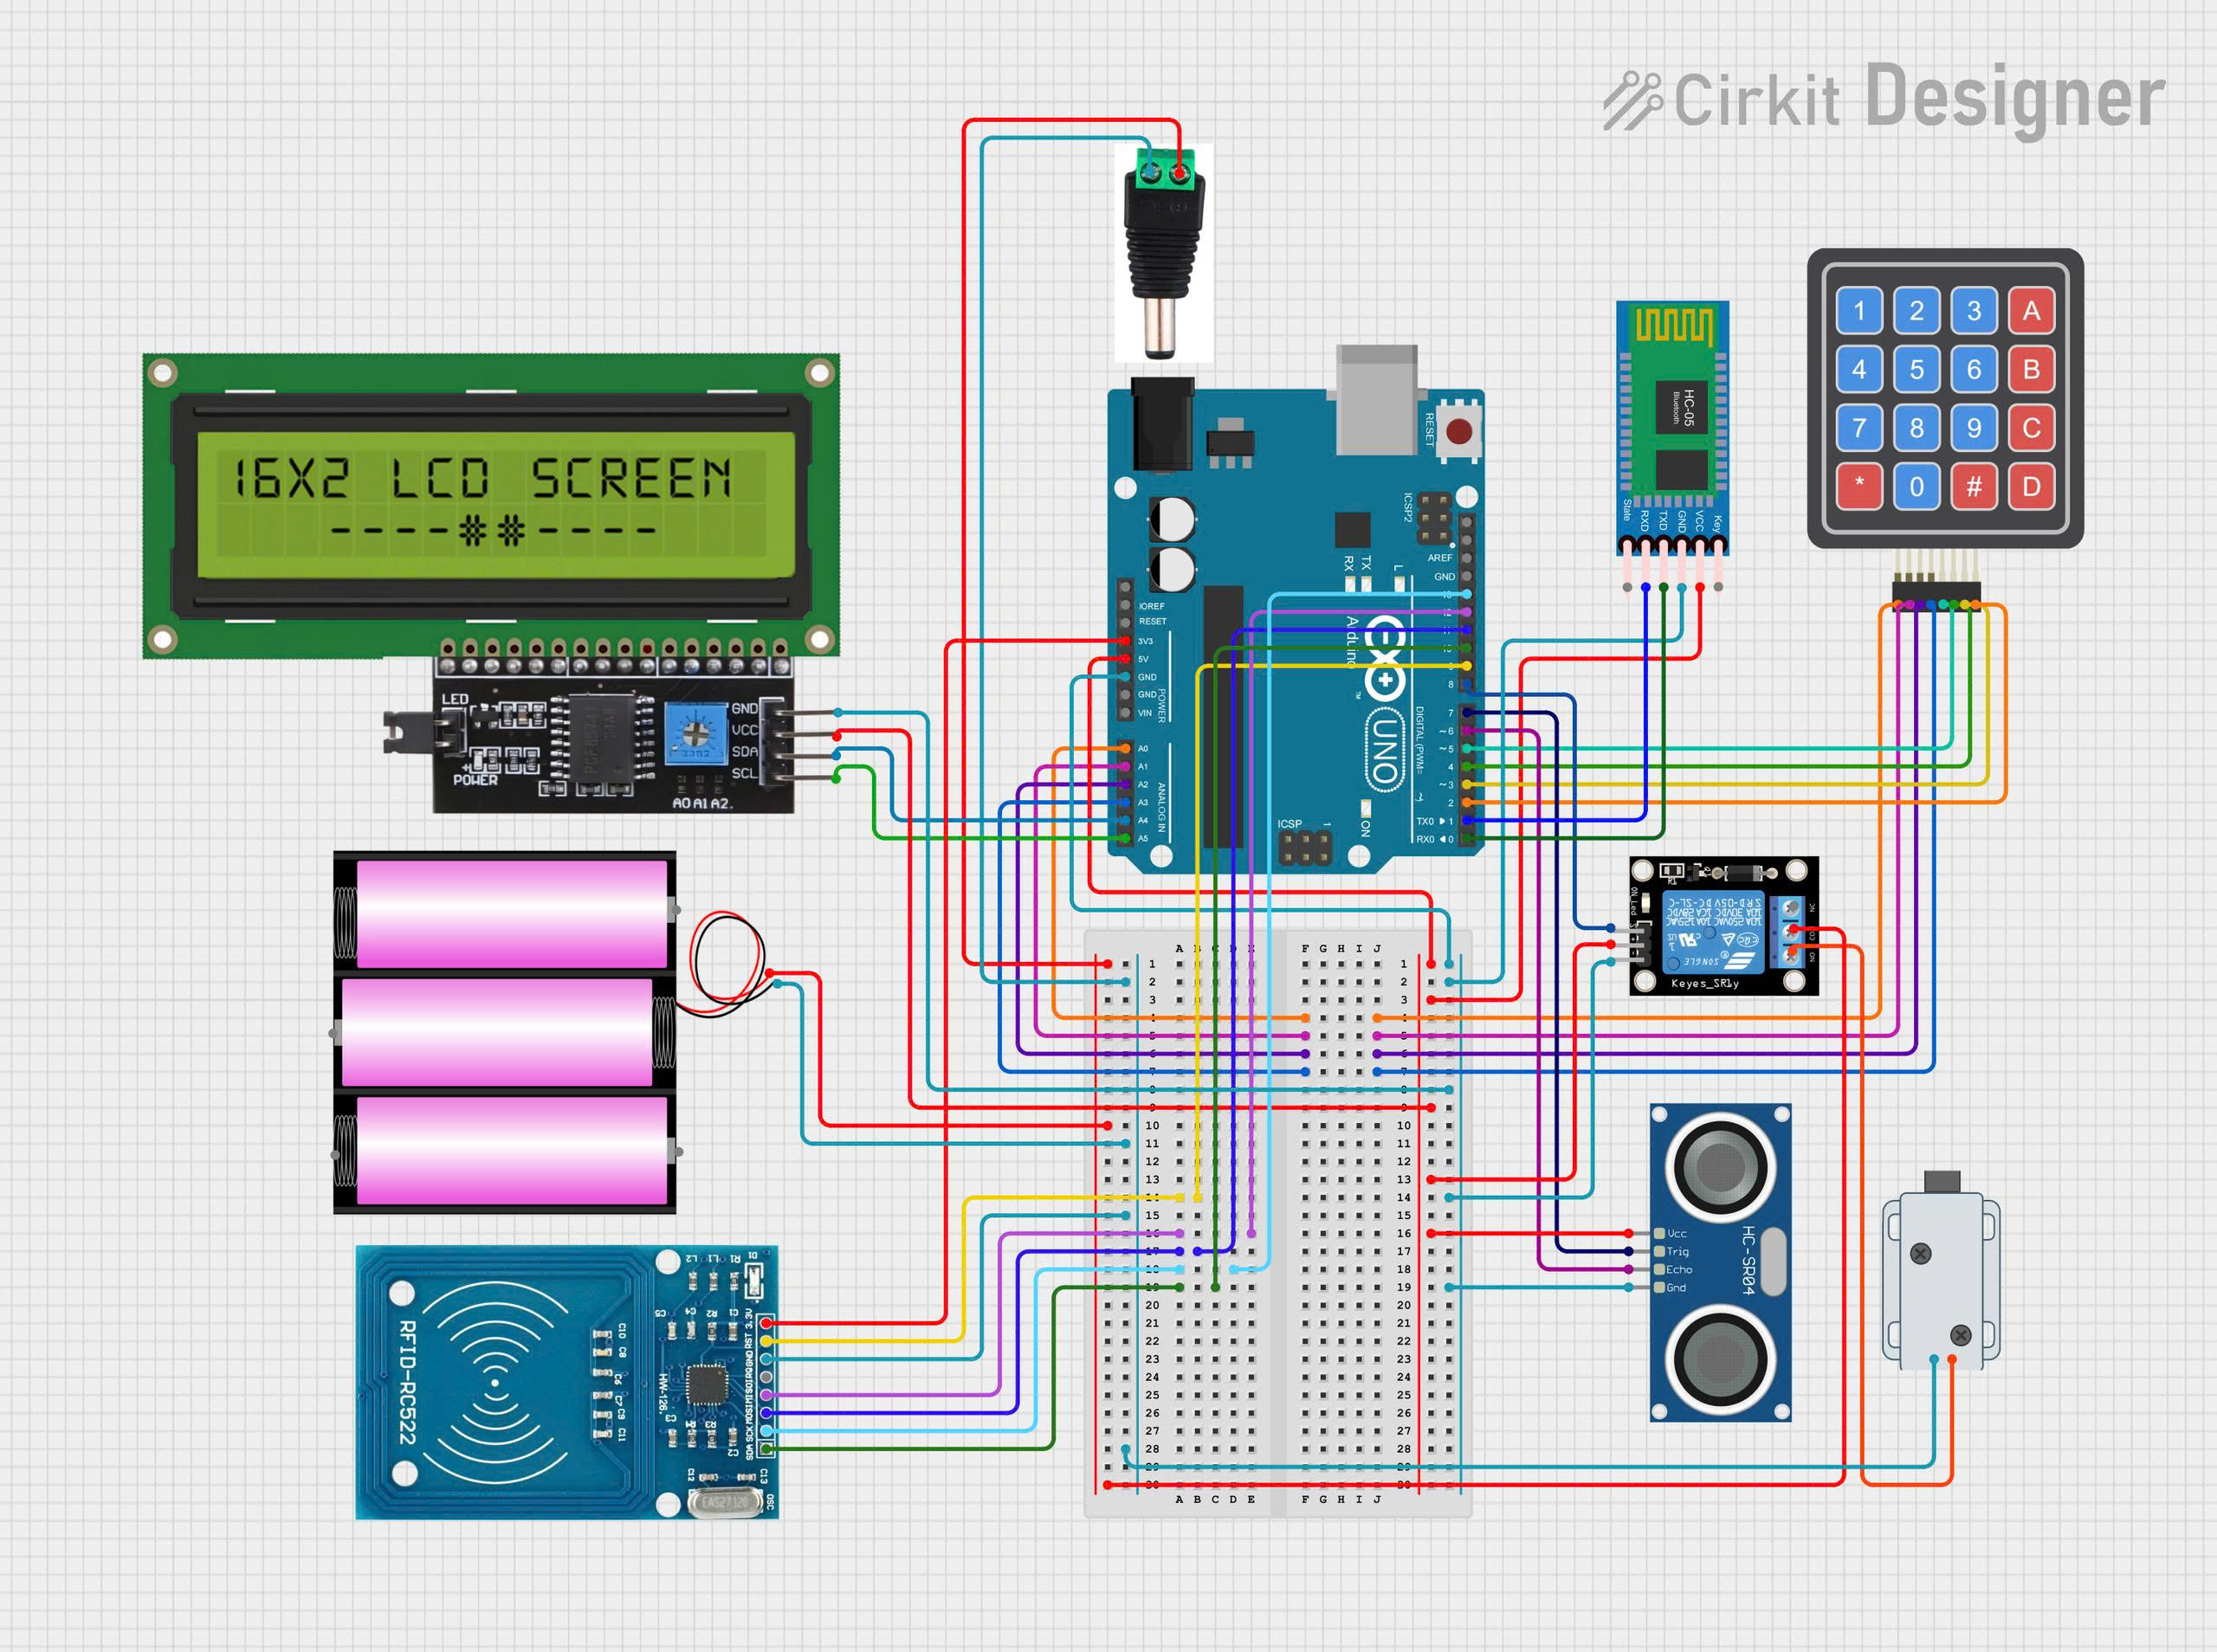
\includegraphics[width=0.65\textwidth]{cri.jpg}
	\caption{Circuit Diagram.}
	\label{fig9}
\end{figure}	


\begin{table}[htb]
	\caption{Interfacing Between Arduino Uno and Components}
	\label{tab:interface_table}
	\centering
	\scriptsize
	\renewcommand{\arraystretch}{1.4}
	\begin{adjustbox}{max width=0.98\textwidth}
		\begin{tabular}{|c|p{2.3cm}|p{2.3cm}|p{2.3cm}|p{2.3cm}|p{2.3cm}|p{2.3cm}|p{2.3cm}|}
			\hline
			\textbf{Pin Type} & \textbf{Ultrasonic Sensor (HC-SR04)} & \textbf{RFID Module (RC522)} & \textbf{4x4 Keypad} & \textbf{Relay Module} & \textbf{Bluetooth Module (HC-05)} & \textbf{LCD 16x2 (I2C)} & \textbf{ESP8266 (NodeMCU)} \\
			\hline
			\textbf{GND} & GND & GND & GND (shared) & GND & GND & GND & GND \\
			\hline
			\textbf{VCC} & 5V & 3.3V & 5V & 5V & 5V & 5V & 3.3V \\
			\hline
			\textbf{Digital I/O} & Trig (D10), Echo (D9) & 
			SDA (D11), SCK (D13), MOSI (D12), MISO (D8), RST (D7) & 
			8 pins (D0–D6, A0) & 
			IN (D4) & 
			TX (D2), RX (D3) via SoftwareSerial & 
			SDA (A4), SCL (A5) & 
			GPIOs D0–D8 (optional control) \\
			\hline
			\textbf{Analog} & – & – & – & – & – & – & A0 (if needed) \\
			\hline
			\textbf{Comm. Protocol} & Digital Pulse & SPI & Matrix Scanning & Digital Output & UART (TX/RX) & I2C & Wi-Fi + GPIO \\
			\hline
		\end{tabular}
	\end{adjustbox}
\end{table}


\subsection{Software Programming}

The Arduino-based smart door lock system developed by Group 2 represents a robust, scalable, and interactive solution for secure access control in modern environments such as homes, offices, and laboratories. The project combines multiple hardware modules, including sensors, actuators, and communication peripherals, all interconnected through well-defined GPIO assignments on the Arduino Uno. Each module has a specific role and is integrated using industry-standard protocols such as UART, SPI, and I2C to ensure reliability, modularity, and ease of maintenance.

\begin{figure}[H]
	\centering
	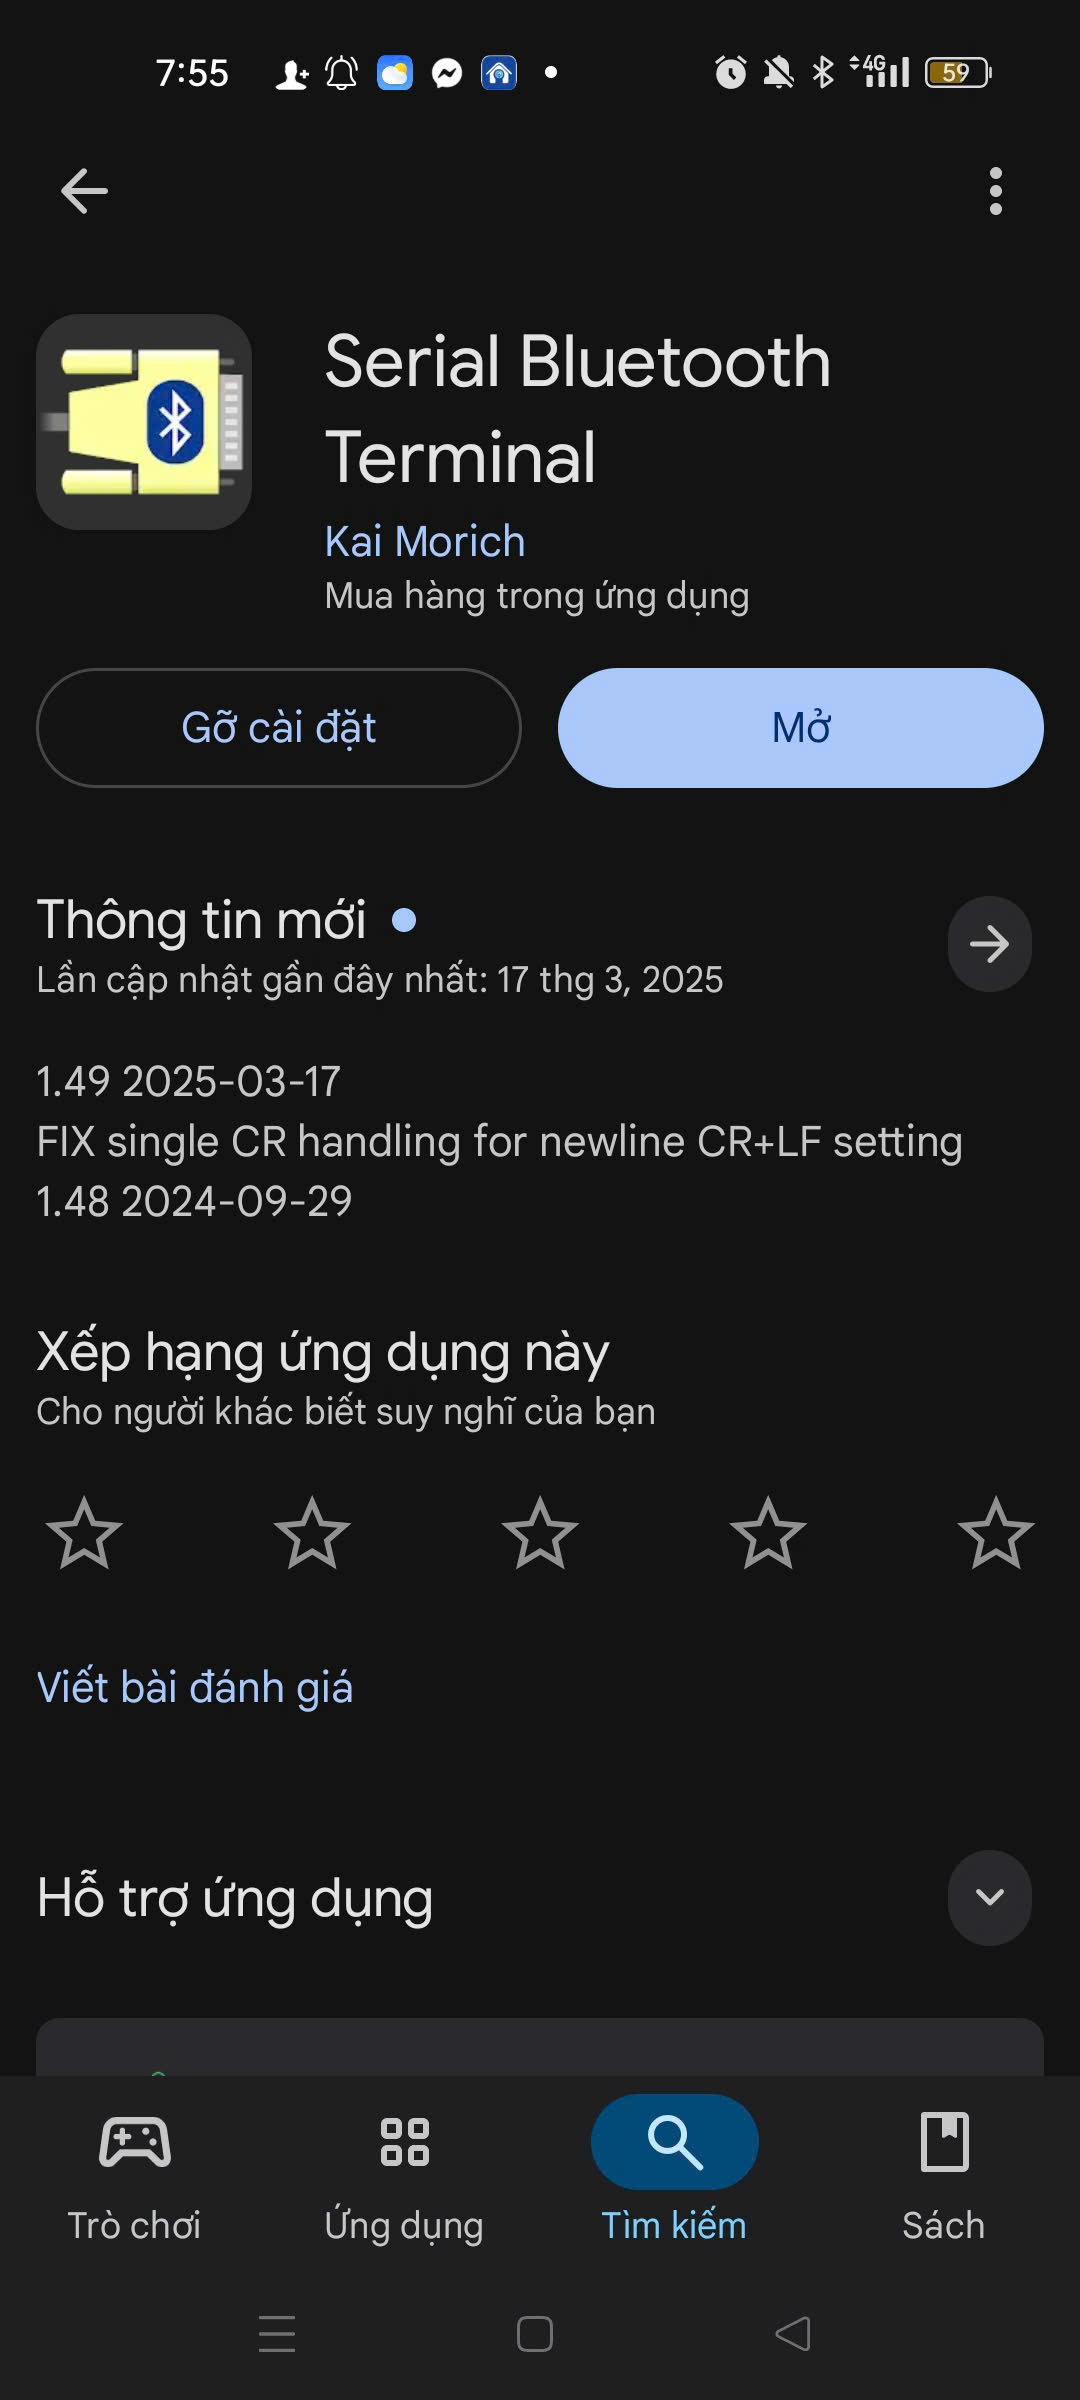
\includegraphics[width=0.2\textwidth]{z6844980615115_5eaad1d876e79f6f298e16e523106730.jpg}
\end{figure}	

At the center of the system is the Arduino Uno R3, which operates as the main controller responsible for real-time monitoring, user authentication, data storage, and decision-making. It is programmed to process various types of inputs and respond accordingly by controlling output devices such as a relay for door locking/unlocking.

\begin{figure}[H]
	\centering
	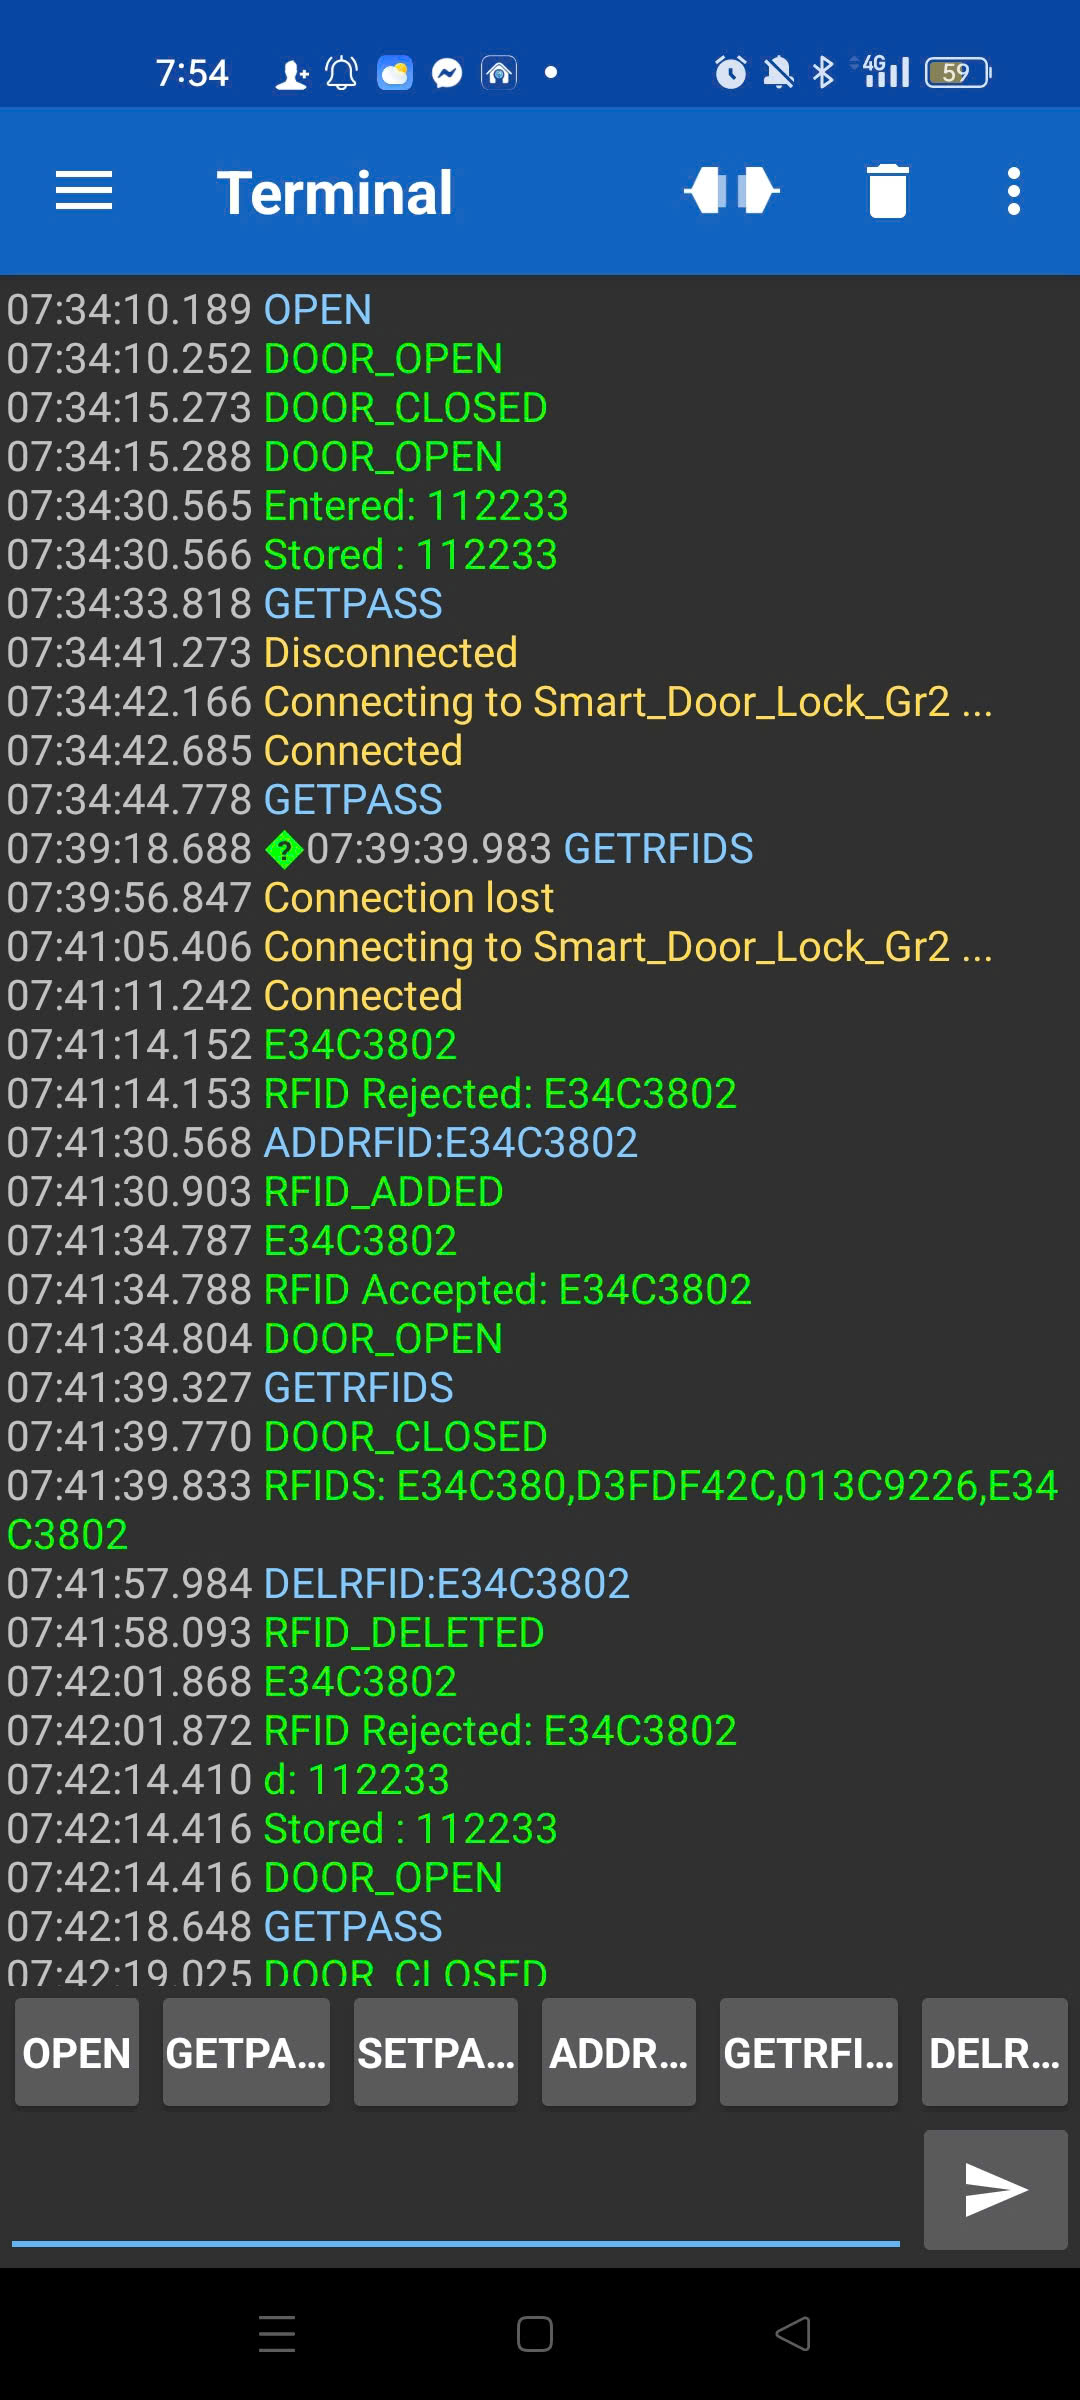
\includegraphics[width=0.2\textwidth]{z6844980631319_ed6547c27e0b4fd7fc6d74ca491227c5.jpg}
\end{figure}

The Ultrasonic sensor (HC-SR04) plays a key role in detecting human presence near the system. It connects to digital pin \texttt{7} (TRIG) and pin \texttt{6} (ECHO), allowing the system to emit and measure sound pulses to calculate distance. When a user approaches within 50 cm, the LCD display is automatically activated, welcoming the user with a prompt for authentication. This sensor-based activation minimizes unnecessary power usage and prolongs LCD lifespan while also enhancing user experience through a responsive interface.

The door's lock is controlled via an electromagnetic relay module, which is connected to digital pin \texttt{8}. The relay acts as a high-power switch capable of toggling the electrical connection to an actual locking mechanism (e.g., solenoid lock or magnetic door lock). The relay is normally set to LOW, which keeps the door locked. Upon successful authentication, the Arduino outputs a HIGH signal to energize the relay for 5 seconds, unlocking the door, after which it automatically returns to the locked state. This ensures both security and automation, eliminating the need for manual locking.

User input is primarily gathered through a 4x4 matrix keypad, which is essential for entering numeric passwords. The keypad's 4 rows are connected to analog pins \texttt{A0} to \texttt{A3}, while the 4 columns are connected to digital pins \texttt{2} to \texttt{5}. This hardware layout allows the system to efficiently scan the matrix for key presses using the \texttt{Keypad.h} library. The use of analog pins for digital input maximizes available GPIO resources and leaves room for future expansion. The keypad supports up to 16 keys, offering flexibility for password entry and control commands.

The system includes an RFID module (MFRC522) to enable contactless access. It is interfaced using the SPI protocol with dedicated pins: \texttt{MOSI (D11)}, \texttt{MISO (D12)}, \texttt{SCK (D13)}, \texttt{SS (D10)}, and \texttt{RST (D9)}. When a user presents an RFID card or tag, the reader retrieves its unique identifier (UID), which is then compared to stored UIDs in EEPROM. If a match is found, access is granted. The module supports reading from standard 13.56 MHz tags, providing a fast and reliable authentication method that complements the keypad.

Wireless interaction is facilitated by the HC-05 Bluetooth module, connected via the Arduino’s hardware serial port (\texttt{TX = pin 1}, \texttt{RX = pin 0}). Through this interface, the system can communicate with mobile devices to receive commands such as \texttt{OPEN}, \texttt{CLOSE}, \texttt{SETPASS}, and RFID management instructions. The integration of Bluetooth provides remote control capabilities, enhancing convenience for users who wish to operate the lock without physically interacting with it.

A 16x2 Liquid Crystal Display (LCD) with I2C interface provides visual feedback to the user. Connected to analog pins \texttt{A4 (SDA)} and \texttt{A5 (SCL)}, it displays messages like “\texttt{LOCKED}”, “\texttt{SUCCESS, UNLOCKED}”, and error prompts. I2C communication reduces the number of GPIO pins required (compared to traditional parallel LCD wiring), simplifying wiring and increasing system modularity.

To ensure the system retains user settings across reboots, the Arduino’s onboard EEPROM memory is utilized for non-volatile storage. The password is stored starting at address \texttt{0}, and RFID card UIDs are stored sequentially starting from address \texttt{10}, with each ID occupying a fixed 8-byte block. This memory structure enables efficient look-up and update operations. The firmware includes dedicated functions to save and load this data during startup, ensuring seamless user experience and robust configuration persistence.

The current design supports up to four RFID users and a 6-digit password. However, the modular architecture makes it easy to scale further. The EEPROM usage can be optimized to support more users, or an external EEPROM or SD card module can be introduced. Similarly, additional features like a fingerprint sensor, buzzer, or internet-based control via ESP8266/ESP32 can be integrated with minimal changes to the code or wiring due to the modular structure and abstraction of hardware layers.

Moreover, the use of standard communication protocols means that each peripheral could be upgraded or replaced without overhauling the entire system. For instance, replacing the LCD with an OLED display or adding a GSM module for SMS alerts would only require minor software adjustments.

In summary, this smart door lock system is a well-architected blend of electronic design and embedded programming. It leverages the full range of the Arduino Uno’s hardware capabilities by distributing I/O tasks across digital, analog, and communication pins in an optimized manner. With multiple authentication methods — including password, RFID, and Bluetooth — the system ensures flexibility, security, and user-friendliness. The clear separation of functional modules, adherence to standard protocols, and robust EEPROM handling make the system not only effective in its current form but also highly adaptable for future upgrades in the evolving landscape of smart home and IoT technologies.

\begin{figure}[H]
	\centering
	% Top row
	\begin{minipage}[b]{0.3\textwidth}
		\centering
		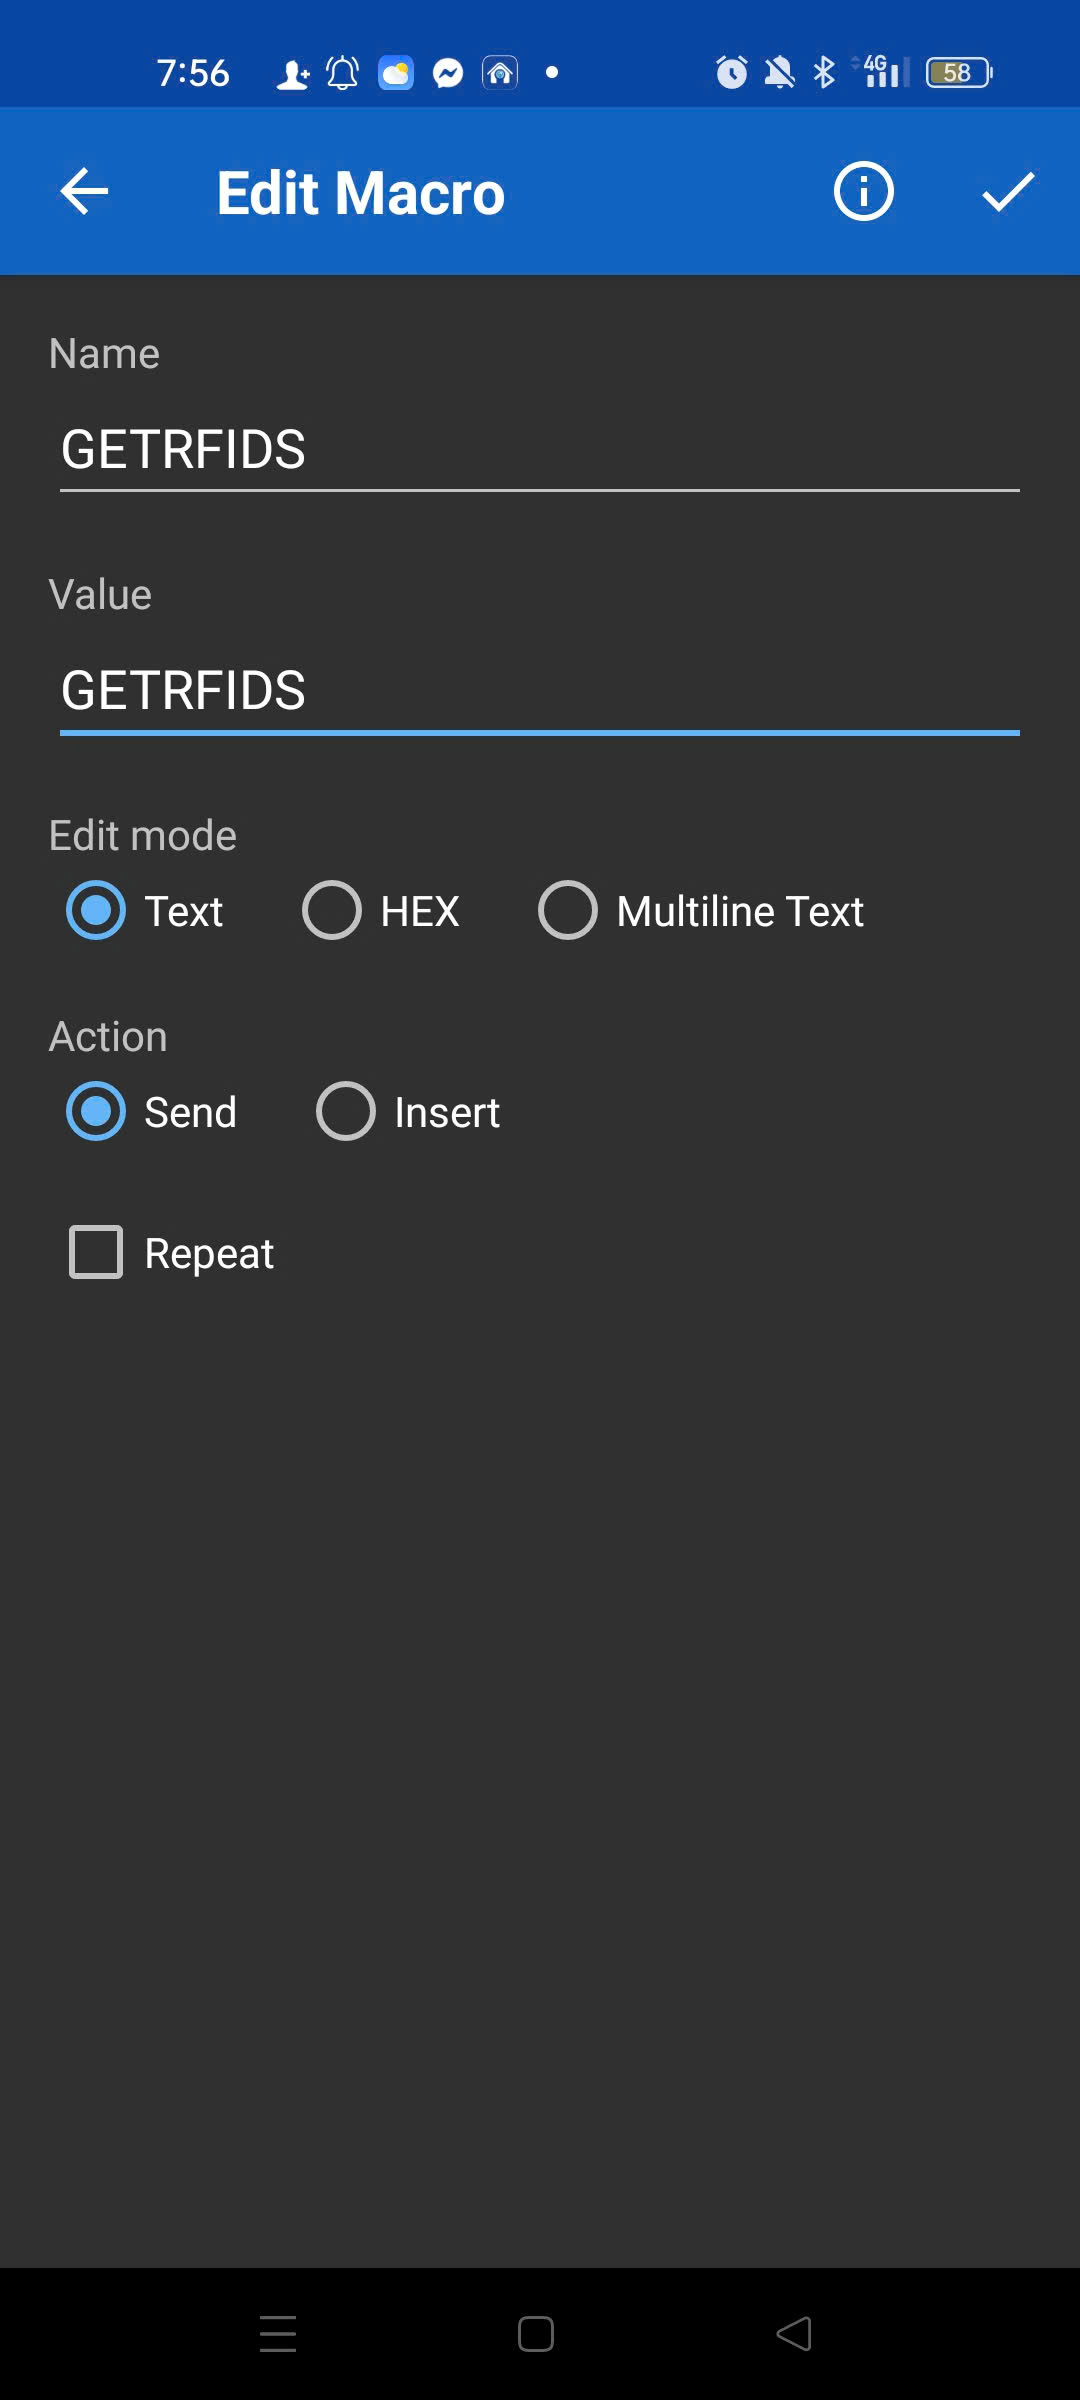
\includegraphics[width=\textwidth]{z6844982585045_becf1e59918c0ba439144229f75b5192.jpg}
	\end{minipage}
	\hspace{0.03\textwidth}
	\begin{minipage}[b]{0.3\textwidth}
		\centering
		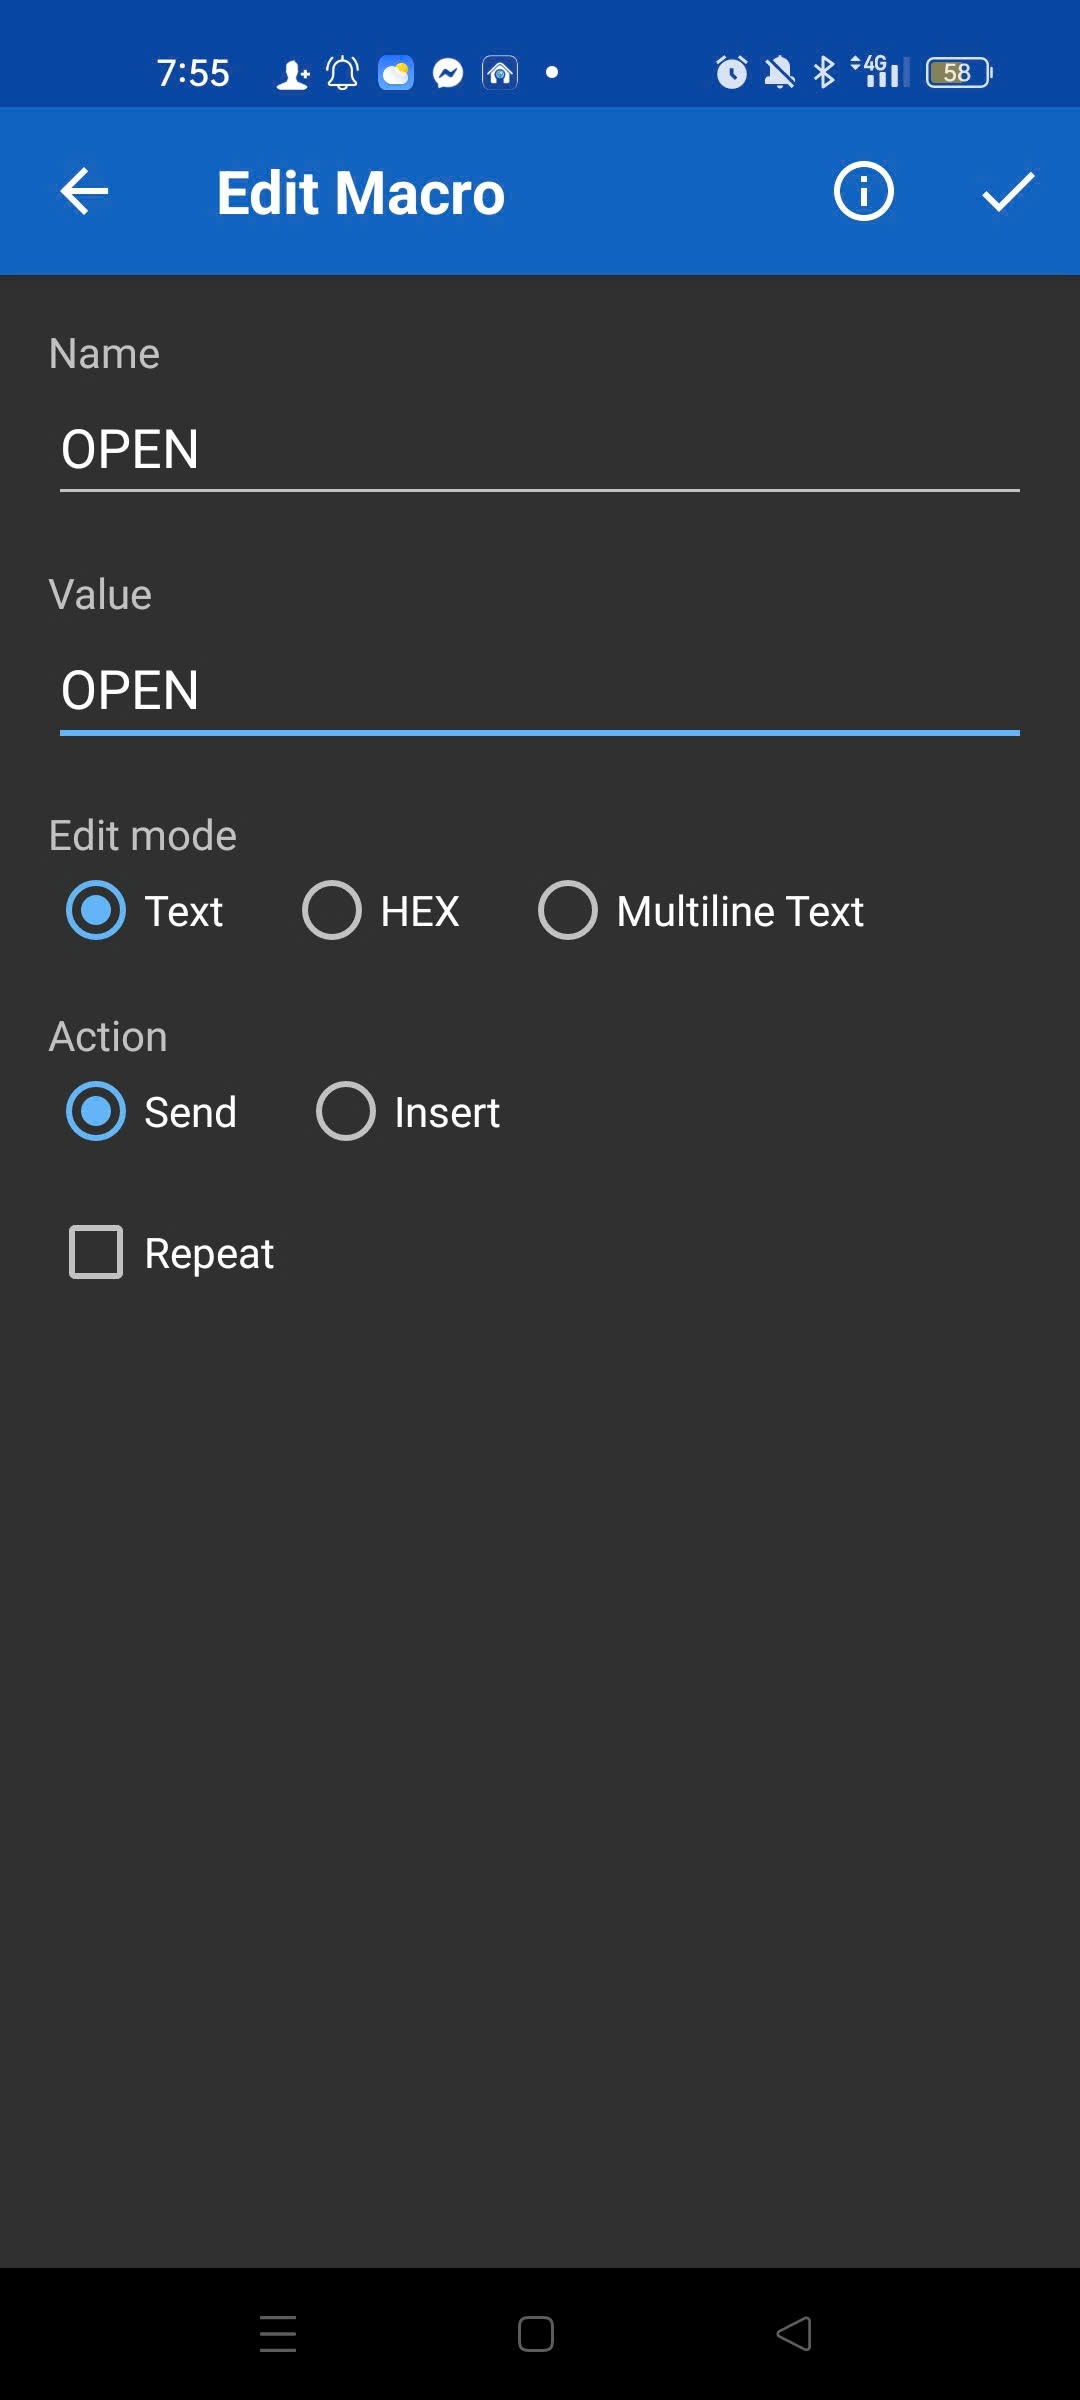
\includegraphics[width=\textwidth]{z6844982521556_dca768482353bb117f4c4fd86b55282d.jpg}
	\end{minipage}
	\hspace{0.03\textwidth}
	\begin{minipage}[b]{0.3\textwidth}
		\centering
		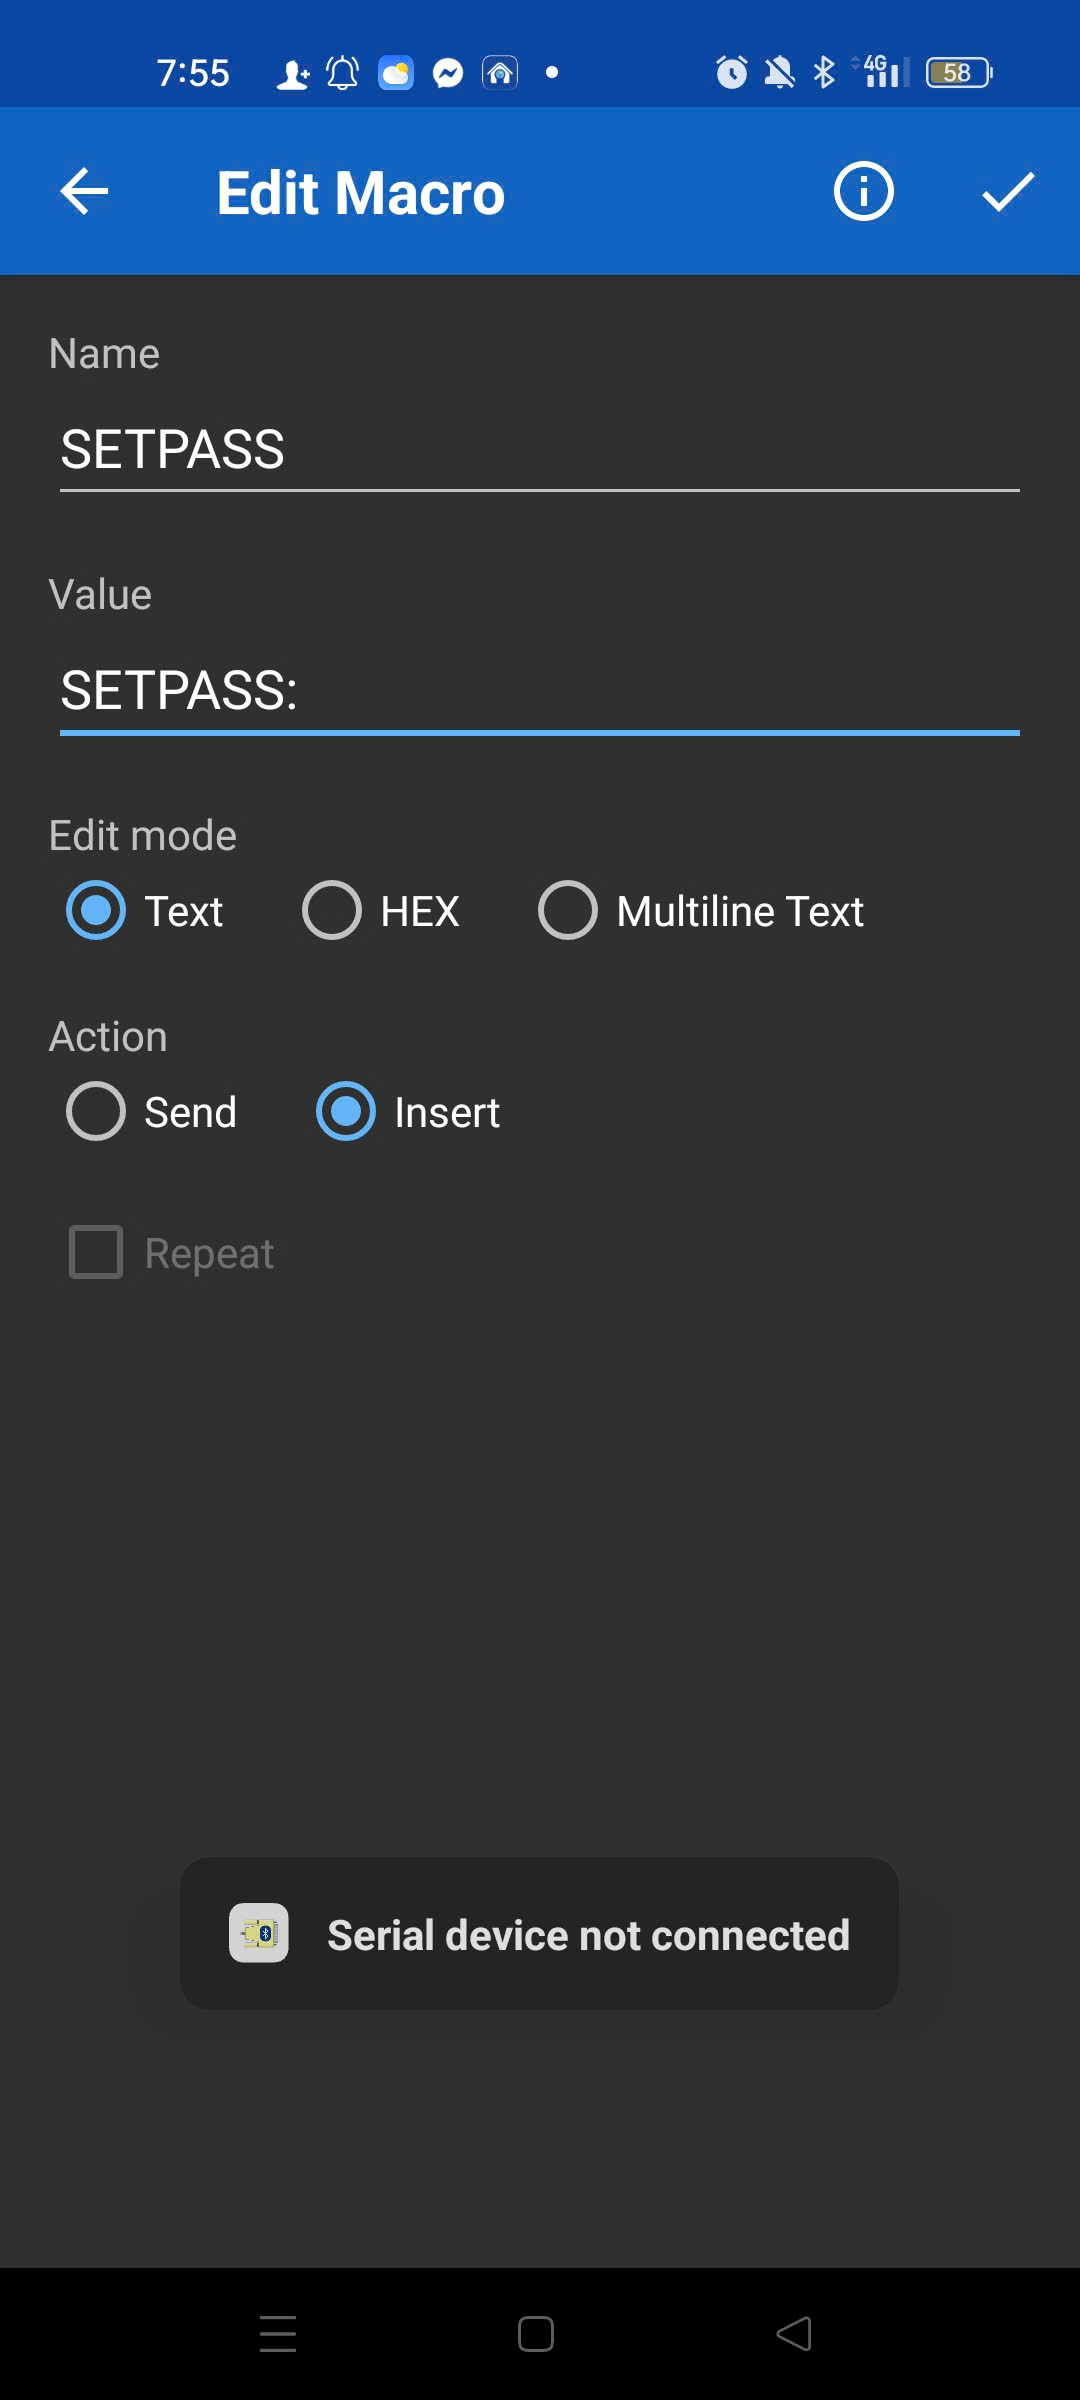
\includegraphics[width=\textwidth]{z6844982516294_bca39df85a16bdcd24fef441729f478a.jpg}
	\end{minipage}
	
	\vspace{0.5cm} % Spacing between rows
	
	% Bottom row
	\begin{minipage}[b]{0.3\textwidth}
		\centering
		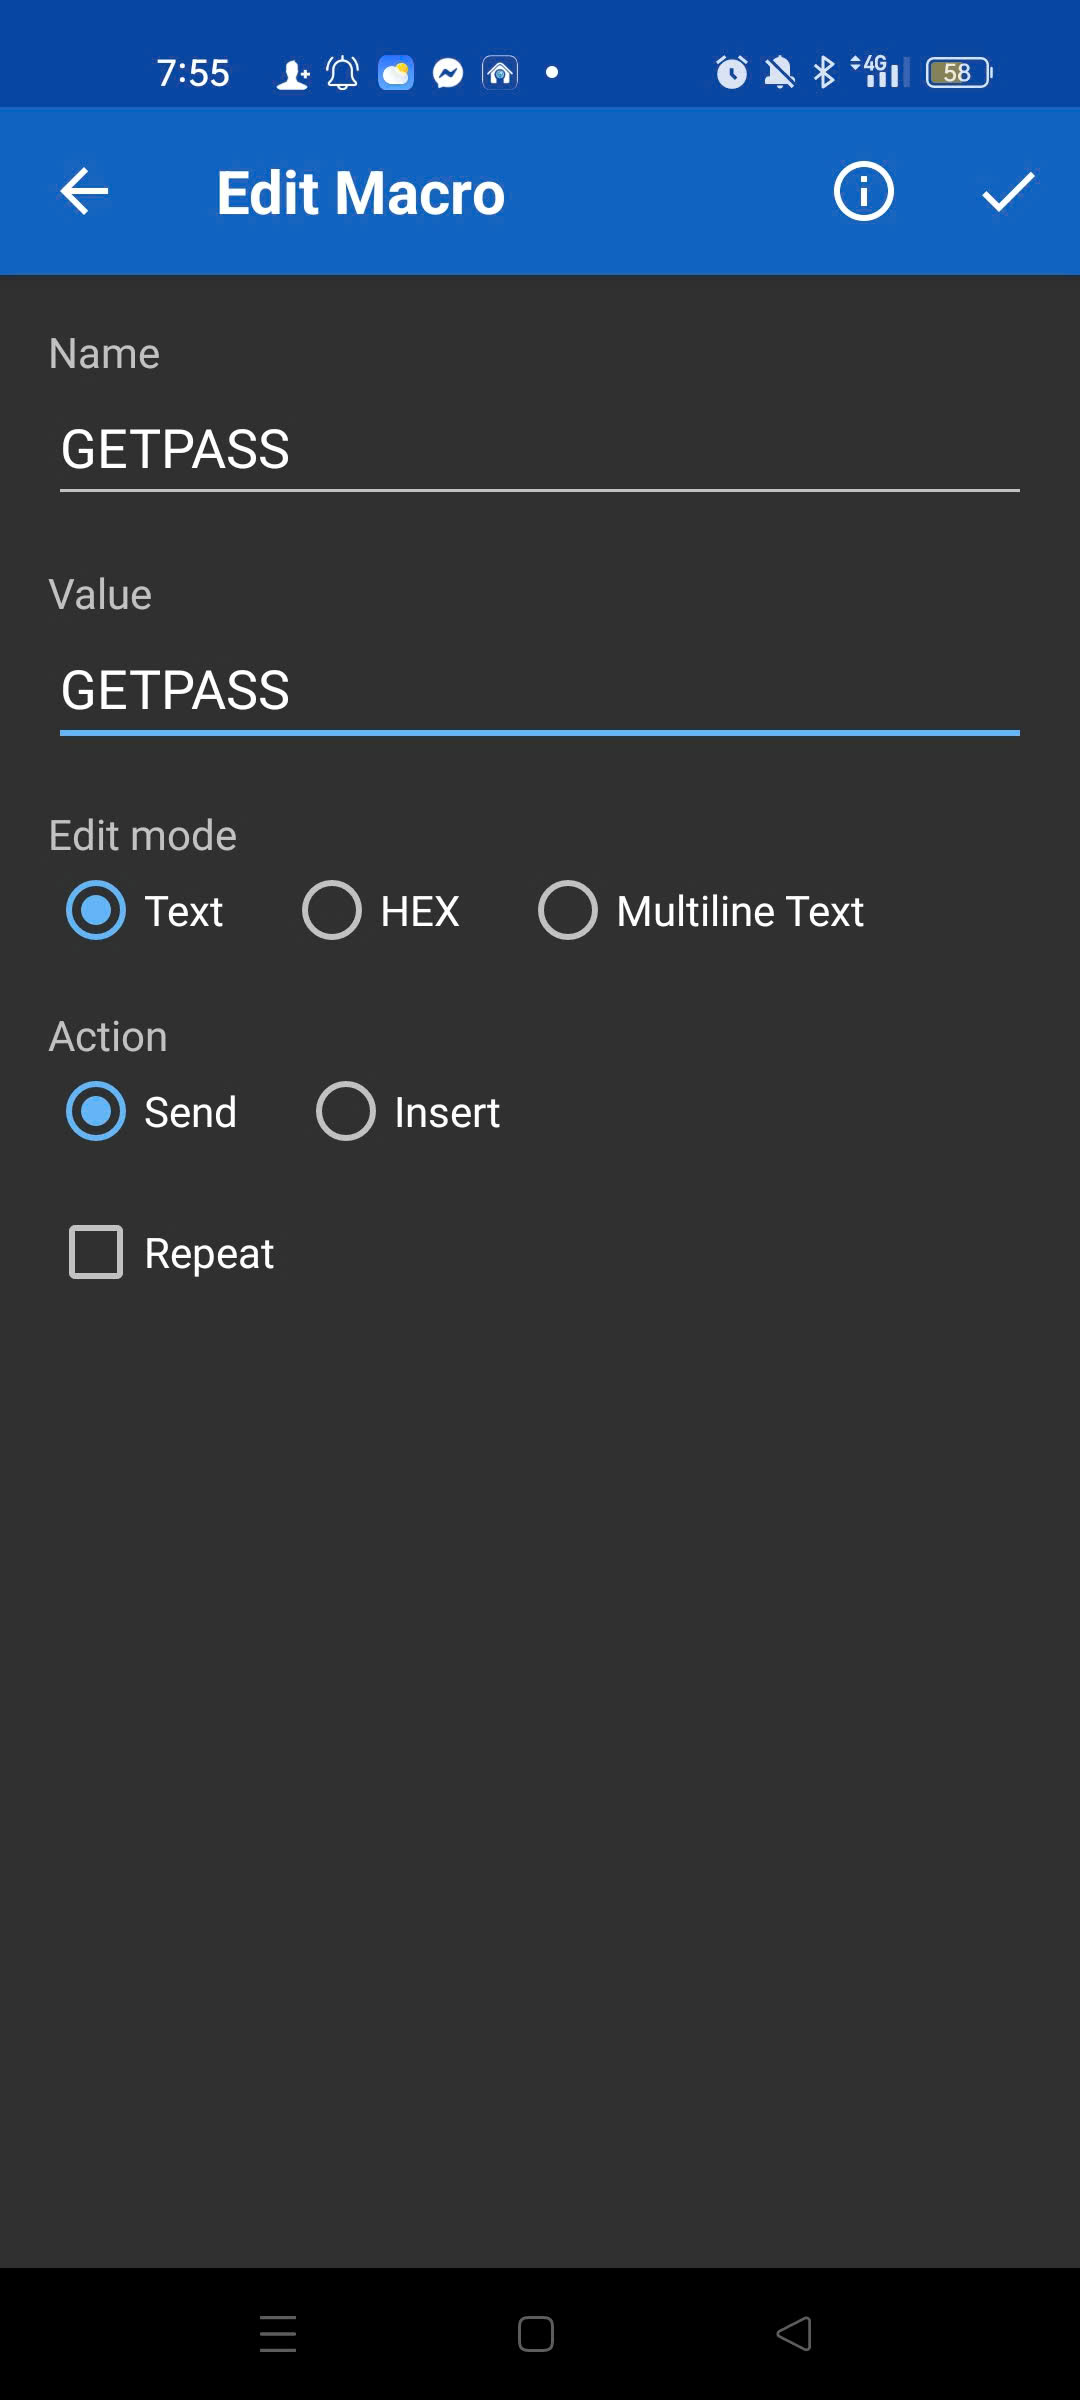
\includegraphics[width=\textwidth]{z6844982508852_47eb2ac8d15c7855521813a8bb1c7e7d.jpg}
	\end{minipage}
	\hspace{0.03\textwidth}
	\begin{minipage}[b]{0.3\textwidth}
		\centering
		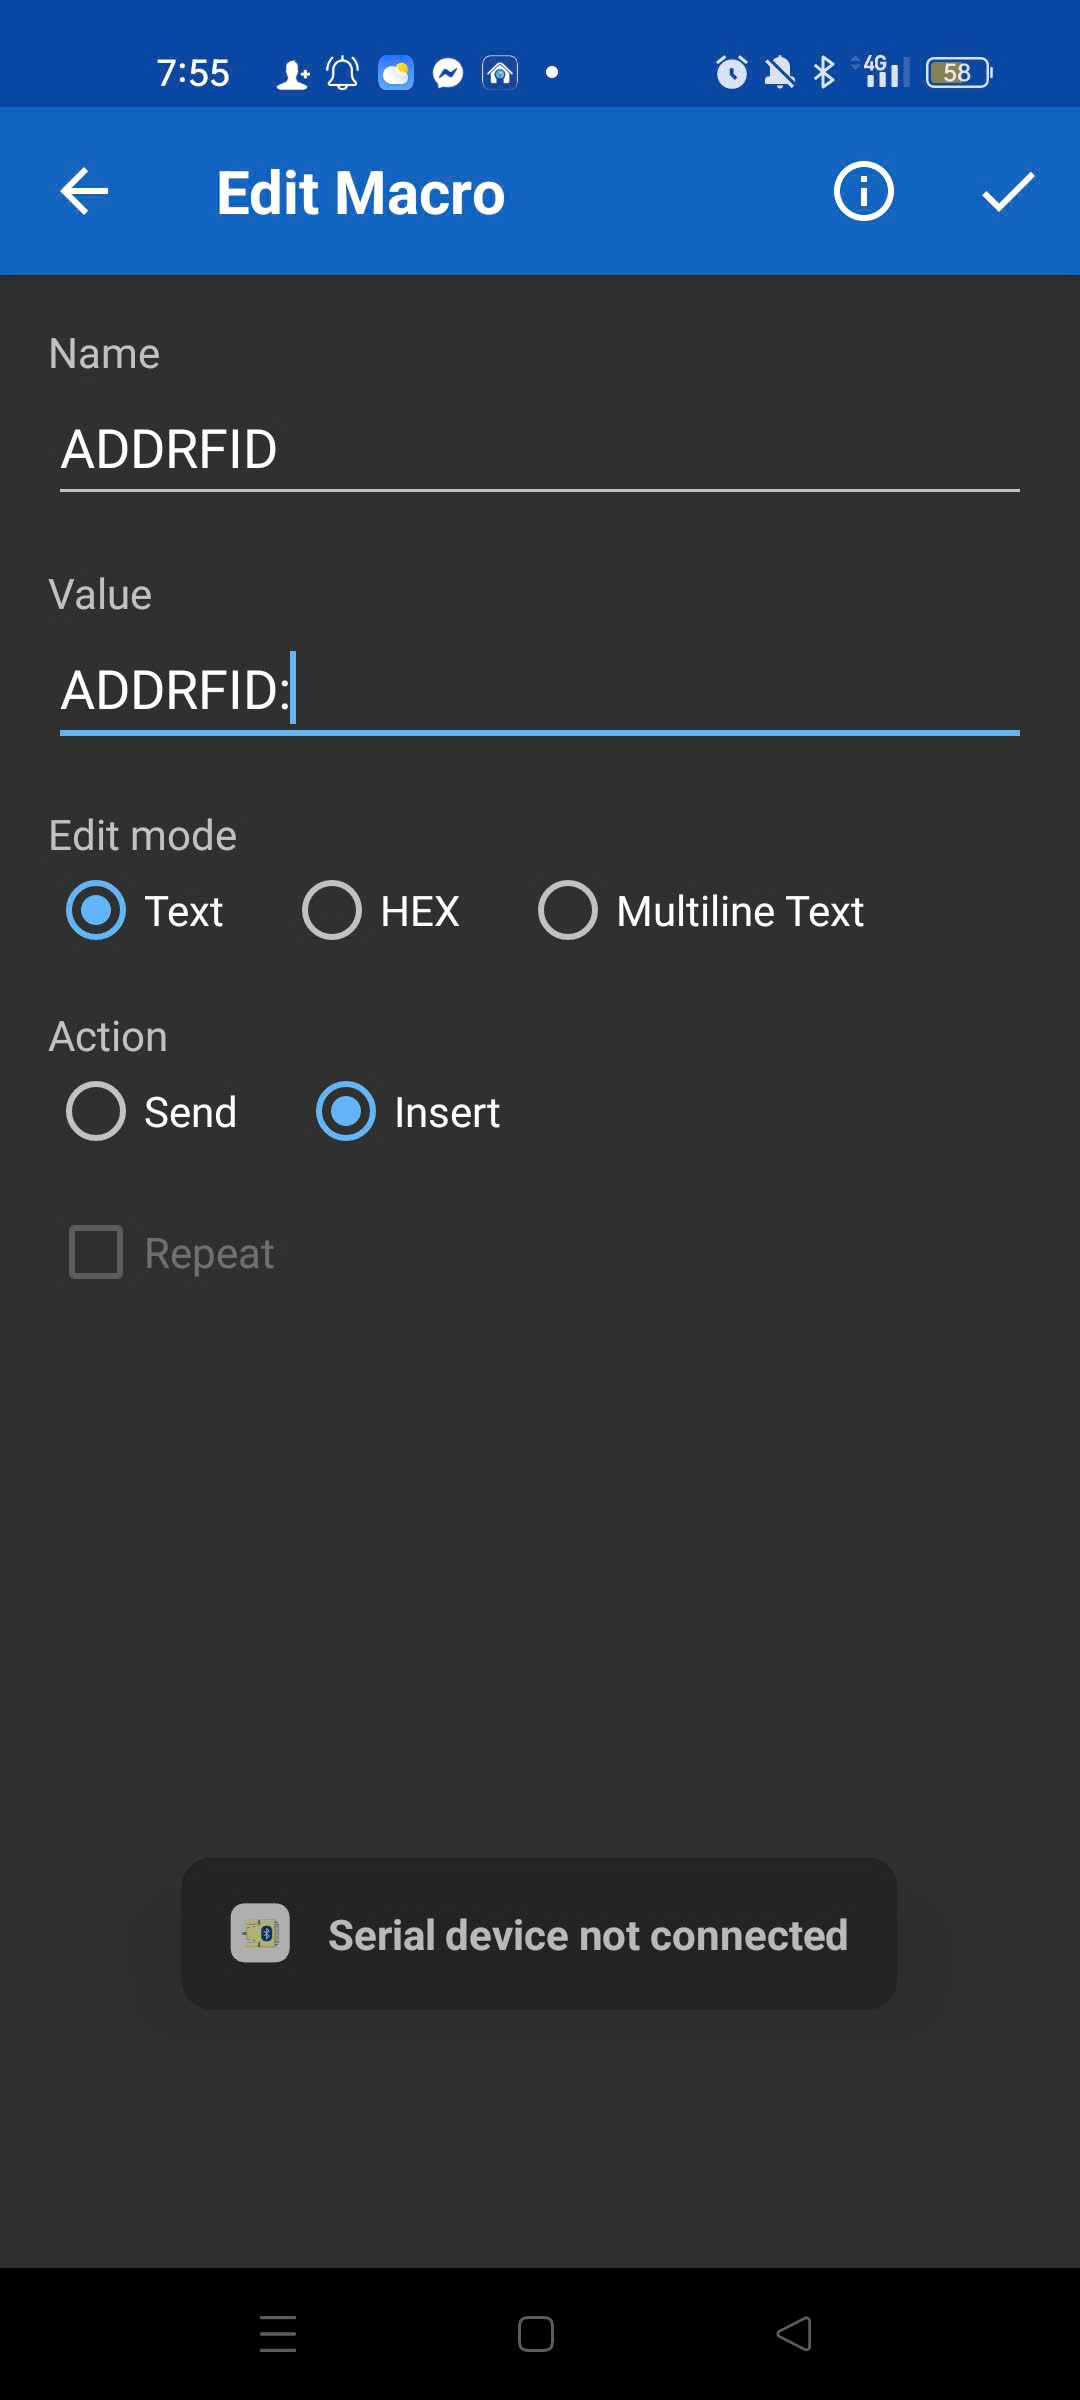
\includegraphics[width=\textwidth]{z6844982506330_f85932b8372ab26a42e4c80e493928d8.jpg}
	\end{minipage}
	\hspace{0.03\textwidth}
	\begin{minipage}[b]{0.3\textwidth}
		\centering
		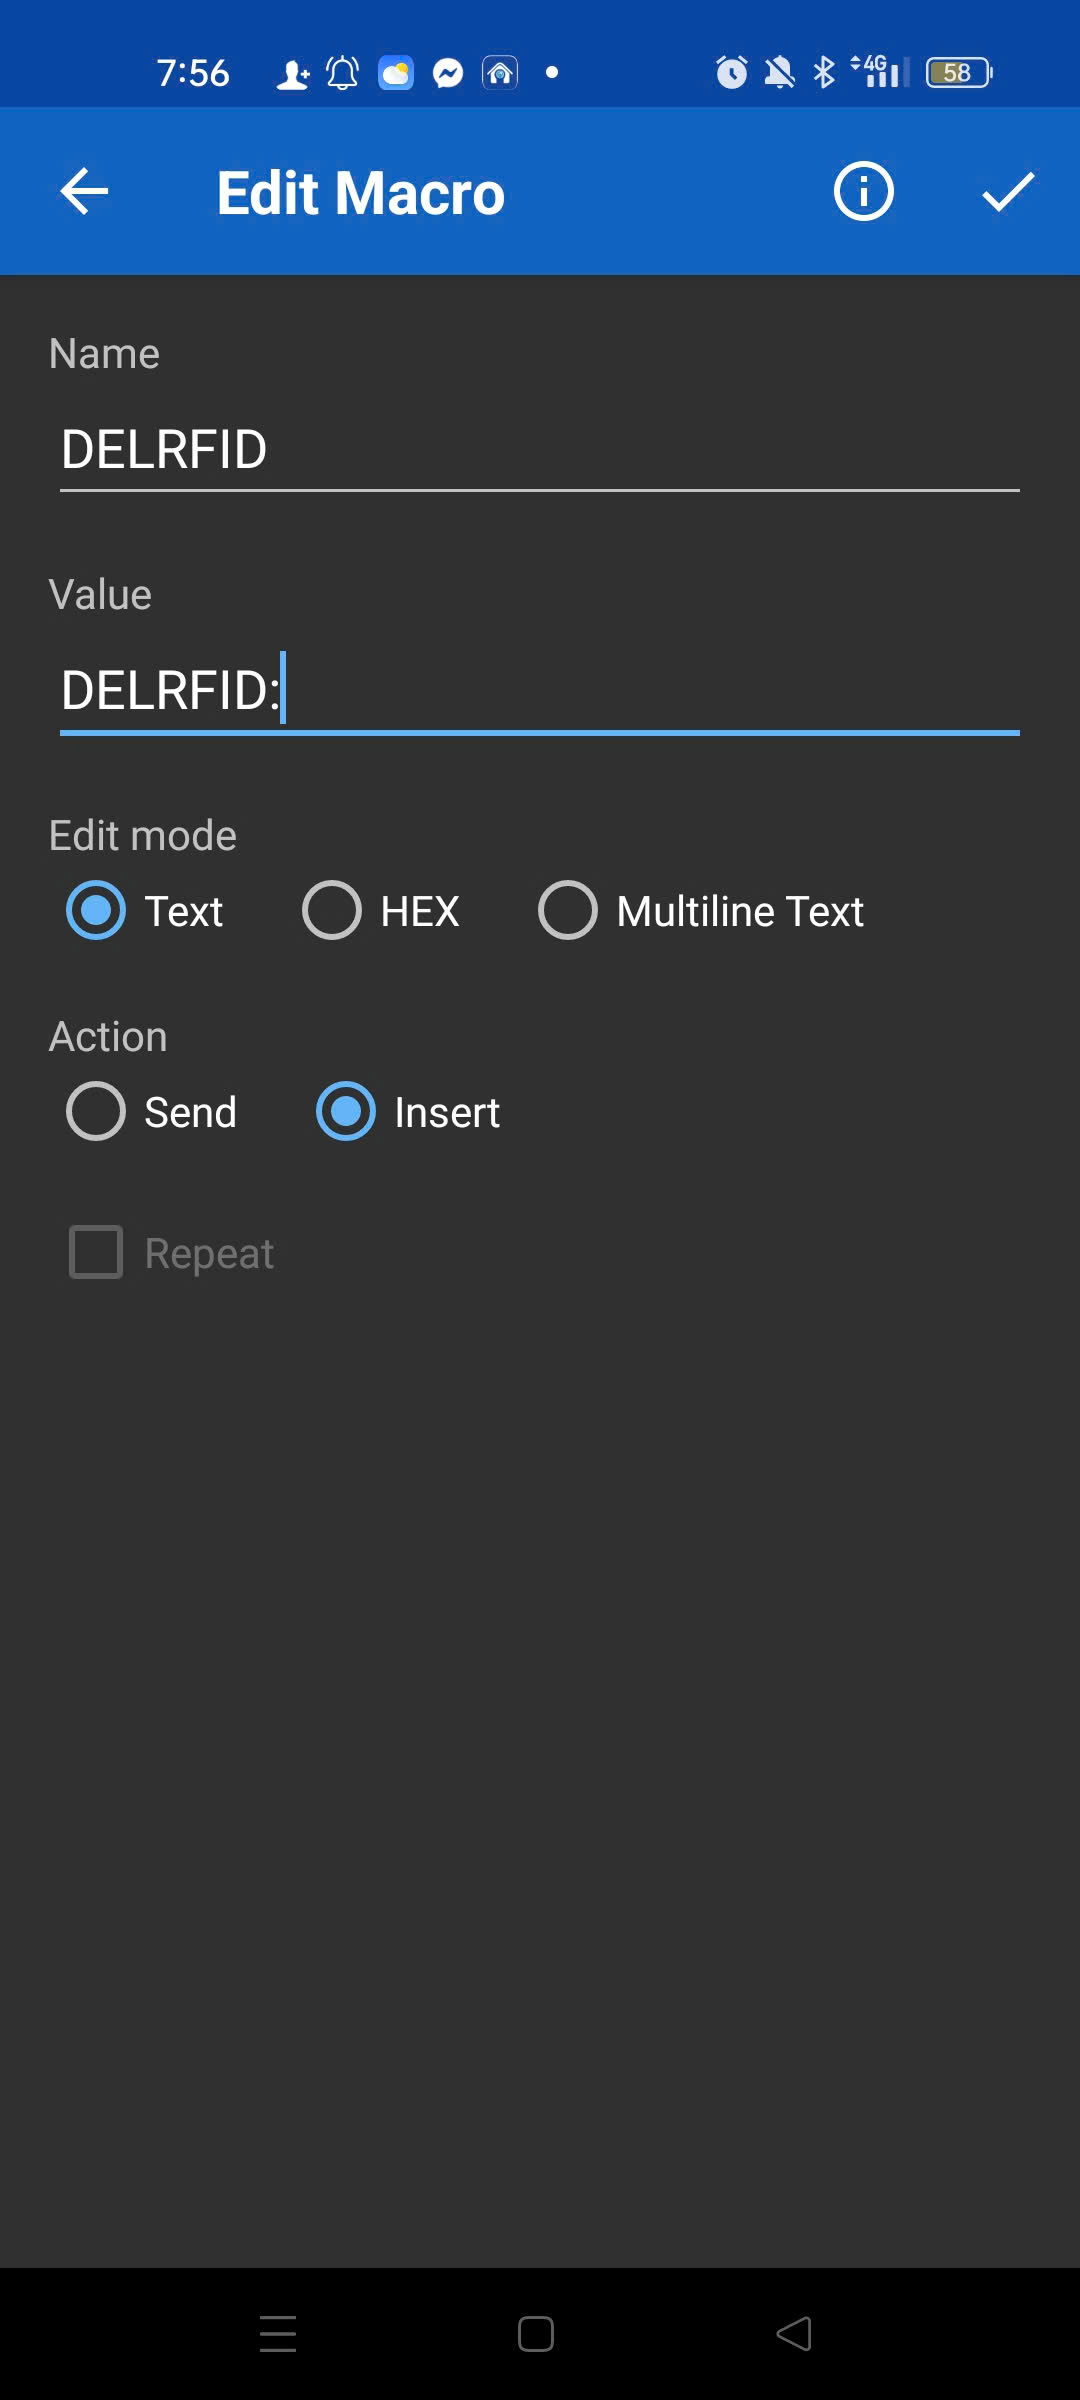
\includegraphics[width=\textwidth]{z6844982497362_0006d2a3461fe6047543e0bac1fd5f71.jpg}
	\end{minipage}
	\caption{Images showing the Software Programming and components of the system}
\end{figure}

\subsection{Programming Flowchart}
\thispagestyle{empty}

% Style definitions
\tikzstyle{startstop} = [rectangle, rounded corners, minimum width=2.2cm, minimum height=0.6cm, text centered, draw=black, fill=white!30]
\tikzstyle{io} = [trapezium, trapezium left angle=70, trapezium right angle=110, minimum width=1.6cm, minimum height=0.6cm, text centered, draw=black, fill=white!30]
\tikzstyle{process} = [rectangle, minimum width=1.9cm, minimum height=0.6cm, text centered, draw=black, fill=white!30]
\tikzstyle{decision} = [diamond, minimum width=2cm, minimum height=1cm, text centered, draw=black, fill=white!30, font=\normalsize]
\tikzstyle{arrow} = [thick,->,>=stealth]


\begin{figure}[H]
	\centering
	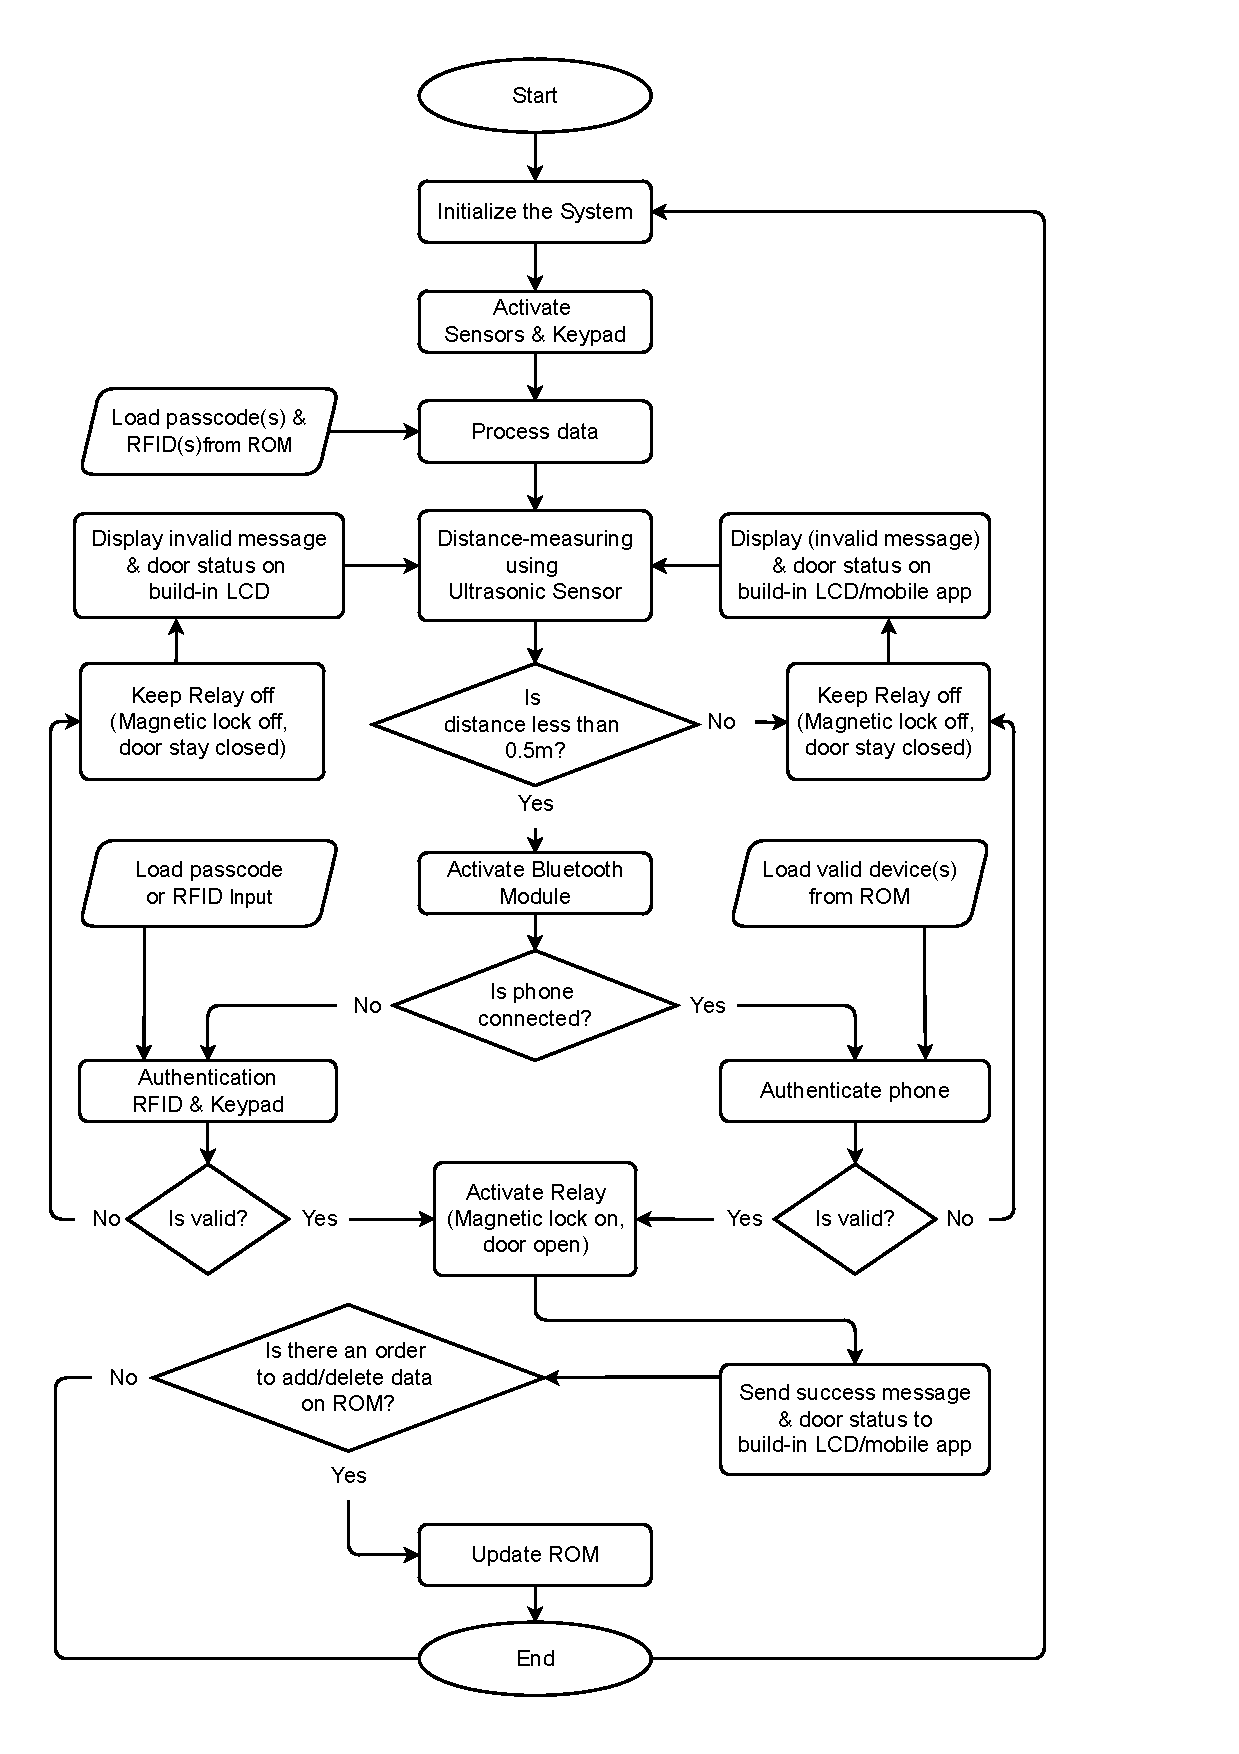
\includegraphics[width=0.65\textwidth]{Untitled Diagram-Page-1.drawio.pdf}
\end{figure}	
The flowchart depicts the complete functional flow of a smart door lock system that employs a layered authentication strategy combining proximity sensing, RFID, keypad input, and Bluetooth-based smartphone verification to ensure secure and efficient access control. Upon powering up, the system enters an initialization phase, during which the microcontroller (e.g., Arduino or ESP8266) prepares the necessary hardware modules, including the ultrasonic distance sensor, RFID reader, 4x4 keypad, Bluetooth module, and internal or external memory (typically EEPROM or flash) that stores authorized user credentials such as passcodes and RFID tags. Once initialized, the system continuously monitors its environment by activating the ultrasonic sensor, which measures the distance of any object (assumed to be a user) approaching the door. If no object is detected within a critical threshold of 0.5 meters, the system remains idle and displays a status message on the local LCD or connected mobile app, while keeping the relay deactivated and the magnetic lock engaged (door locked). However, when a valid presence is detected within range, the system proceeds to activate the Bluetooth communication module and simultaneously allows for user interaction through the keypad or RFID reader. At this stage, two parallel authentication paths are supported: one through physical input (entering a PIN code or scanning an RFID card), and the other via wireless pairing with a smartphone application, which can be authenticated by checking the device’s ID against a list of valid entries stored in ROM. The system performs credential verification in real-time—if the input is deemed valid in either path, it sends a command to activate the relay module, thereby powering the 12~V electromagnetic lock and unlocking the door. The system then displays a success message and updates the access status on both the LCD and the smartphone app. In the event of an invalid attempt, the system simply maintains the locked state, displays an error message, and resets to await further input. Furthermore, if a valid user requests to modify the list of authorized credentials (such as adding or deleting a passcode or RFID), the system temporarily enters a ROM update mode, securely writing the new data before returning to its default operational loop. This design not only ensures robust physical security but also allows for real-time control, remote access, and administrative scalability, aligning with best practices in IoT-enabled smart home systems. It also reflects a thoughtful power management strategy, where energy-intensive modules like Bluetooth and the relay are only activated conditionally, preserving battery life and improving system longevity in off-grid scenarios. Overall, the flowchart demonstrates a highly modular and event-driven control structure that integrates user interaction, environmental sensing, secure logic flow, and feedback mechanisms in a coherent and efficient manner.

\section{Results and Discussion}
\subsection{Prototype Implementation}
The prototype implementation of the Arduino-based smart door lock system was constructed with careful attention to both hardware integration and software functionality. The system was developed on a standard breadboard platform during the testing phase, followed by semi-permanent assembly on a prototyping board to ensure greater mechanical stability and clearer wire management.
At the core is the Arduino Uno microcontroller, powered via USB or an external 5V DC adapter for improved current stability, particularly important for components like the relay and RFID reader. The HC-SR04 ultrasonic sensor was mounted on the top front of the chassis to detect user presence within a 50 cm radius. When proximity is detected, the system wakes from idle mode and activates the 16x2 LCD screen via I2C communication on pins A4 (SDA) and A5 (SCL). This display provides real-time feedback including welcome messages, password prompts, and access status indicators.
The 4x4 matrix keypad was mounted on the housing and connected to analog pins A0–A3 (rows) and digital pins 2–5 (columns). The keypad enables secure 6-digit password input, which is masked on the LCD with asterisks. Input is verified against a stored password in EEPROM (starting at address 0). In parallel, an MFRC522 RFID reader module was attached to the front panel, interfaced via SPI on pins D11 (MOSI), D12 (MISO), D13 (SCK), D10 (SS), and D9 (RST). It reads RFID card UIDs and matches them with authorized entries in EEPROM (stored starting at address 10).
The electromagnetic relay (controlled through digital pin 8) acts as the intermediary between the system and the locking mechanism. When access is granted, the relay triggers a 12V electromagnetic lock, unlocking the door temporarily for 5 seconds before automatically securing it again.
Additionally, the system incorporates an HC-05 Bluetooth module for wireless control and configuration, connected to the Arduino's hardware serial pins (D0 and D1). A mobile application communicates via Bluetooth using predefined commands such as \texttt{"OPEN"}, \texttt{"SETPASS:xxxxxx"}, or \texttt{"ADDRFID:xxxxxxxx"}, allowing dynamic control and management of credentials.
The firmware was written and uploaded using the Arduino IDE, with support from key libraries such as \texttt{Keypad.h}, \texttt{MFRC522.h}, \texttt{EEPROM.h}, \texttt{SoftwareSerial.h}, and \texttt{LiquidCrystal\_I2C.h}. Modular functions were created to manage authentication logic, EEPROM read/write operations, and LCD display handling.
The entire prototype was tested under various scenarios including correct and incorrect password/RFID inputs, Bluetooth commands, and power loss situations to ensure system reliability and data persistence. This implementation demonstrates a fully functional and scalable IoT-based smart lock solution, suitable for residential or institutional security systems.

\subsection{Experimental Results}

To assess the practical viability of the Arduino-based smart door lock system, a series of comprehensive experiments were conducted under controlled conditions simulating real-world environments. The experimental phase focused on evaluating the performance of individual hardware modules, overall system integration, user interaction efficiency, latency, reliability, and stability across various use cases. The prototype was installed on a simulated wooden door frame, integrating all essential components such as the Arduino Uno R3, MFRC522 RFID module, 4x4 matrix keypad, HC-05 Bluetooth module, HC-SR04 ultrasonic sensor, I2C 16x2 LCD, electromagnetic relay, EEPROM memory, and a servo-based locking mechanism. Power was supplied either via a 5V wall adapter or a 5000 mAh power bank to replicate continuous and portable usage scenarios.

The presence detection functionality was tested using the HC-SR04 ultrasonic sensor, configured to activate the system interface (LCD) when a user approached within 50 cm. Across 50 trials at various angles and environmental conditions, the sensor achieved a 96\% accuracy rate, with minor false positives (4\%) attributed to small objects or pets. The LCD activation occurred within an average of 600 milliseconds, proving adequate for responsive human interaction and contributing to energy efficiency by keeping the display off when idle.

Keypad-based password authentication was tested for accuracy, input reliability, and latency. Using a 6-digit password input through the matrix keypad, the system demonstrated a 100\% key recognition rate, with an overall 98\% success rate for full password validation. Failures were primarily due to delayed or partial inputs. The average time from entering the last digit to system response was approximately 1.2 seconds. Additional features such as backspace and reset improved usability and reduced user error.

RFID-based access control, implemented via the MFRC522 module, was also rigorously evaluated. Four authorized RFID cards were stored in EEPROM for validation. During testing, the reader accurately detected cards within a 3.5 cm range, with optimal recognition below 3 cm. The average response time was under 300 milliseconds, and all 30 attempts with unauthorized cards were correctly denied. These results affirmed the RFID system's reliability, security, and suitability for contactless authentication.

Bluetooth functionality, powered by the HC-05 module, enabled remote operation through serial communication with a smartphone application. Supported commands included \texttt{OPEN}, \texttt{SETPASS}, \texttt{ADDUID}, and \texttt{RESET}. The pairing process was successful in all cases, typically taking around 5 seconds. Command recognition and execution maintained a 98\% success rate, with a latency of approximately 1.5 seconds from command dispatch to action completion. Invalid commands were gracefully handled, with clear feedback displayed on the LCD. This wireless feature significantly enhanced accessibility and user convenience, especially in emergency or remote unlock scenarios.

Relay control and door lock activation were tested to ensure electrical safety and mechanical reliability. The relay module, connected to digital pin 8, switched within 100 milliseconds and consistently activated the locking mechanism over 100 cycles. No overheating, contact bounce, or misfires were observed. The relay automatically returned to its locked (LOW) state after a 5-second unlock duration, ensuring secure access control without requiring user intervention.

The full system integration was validated by concurrently operating multiple modules—ultrasonic, keypad, RFID, Bluetooth, LCD, and EEPROM—without triggering crashes or data conflicts. Over a 3-hour continuous runtime, the system maintained 100\% uptime with stable multitasking across various communication protocols (SPI for RFID, I2C for LCD, UART for Bluetooth, and digital interrupts for keypad and sensors). EEPROM operations were also tested for persistence, storing the password and RFID UIDs in structured address blocks. Data retrieval after power cycles was flawless, and write operations averaged 2 milliseconds per byte, with complete boot-up configurations loaded in under 150 milliseconds.

Power consumption was analyzed using a USB multimeter under three system states: idle, active, and unlock. Idle current draw remained at ~70 mA, increased to ~120 mA during sensor and LCD activation, and peaked at ~180 mA during lock toggling. These metrics suggest that a 5000 mAh battery pack could support continuous moderate use for up to 24 hours, confirming suitability for mobile or solar-powered setups.

\begin{figure}[H]
	\centering
	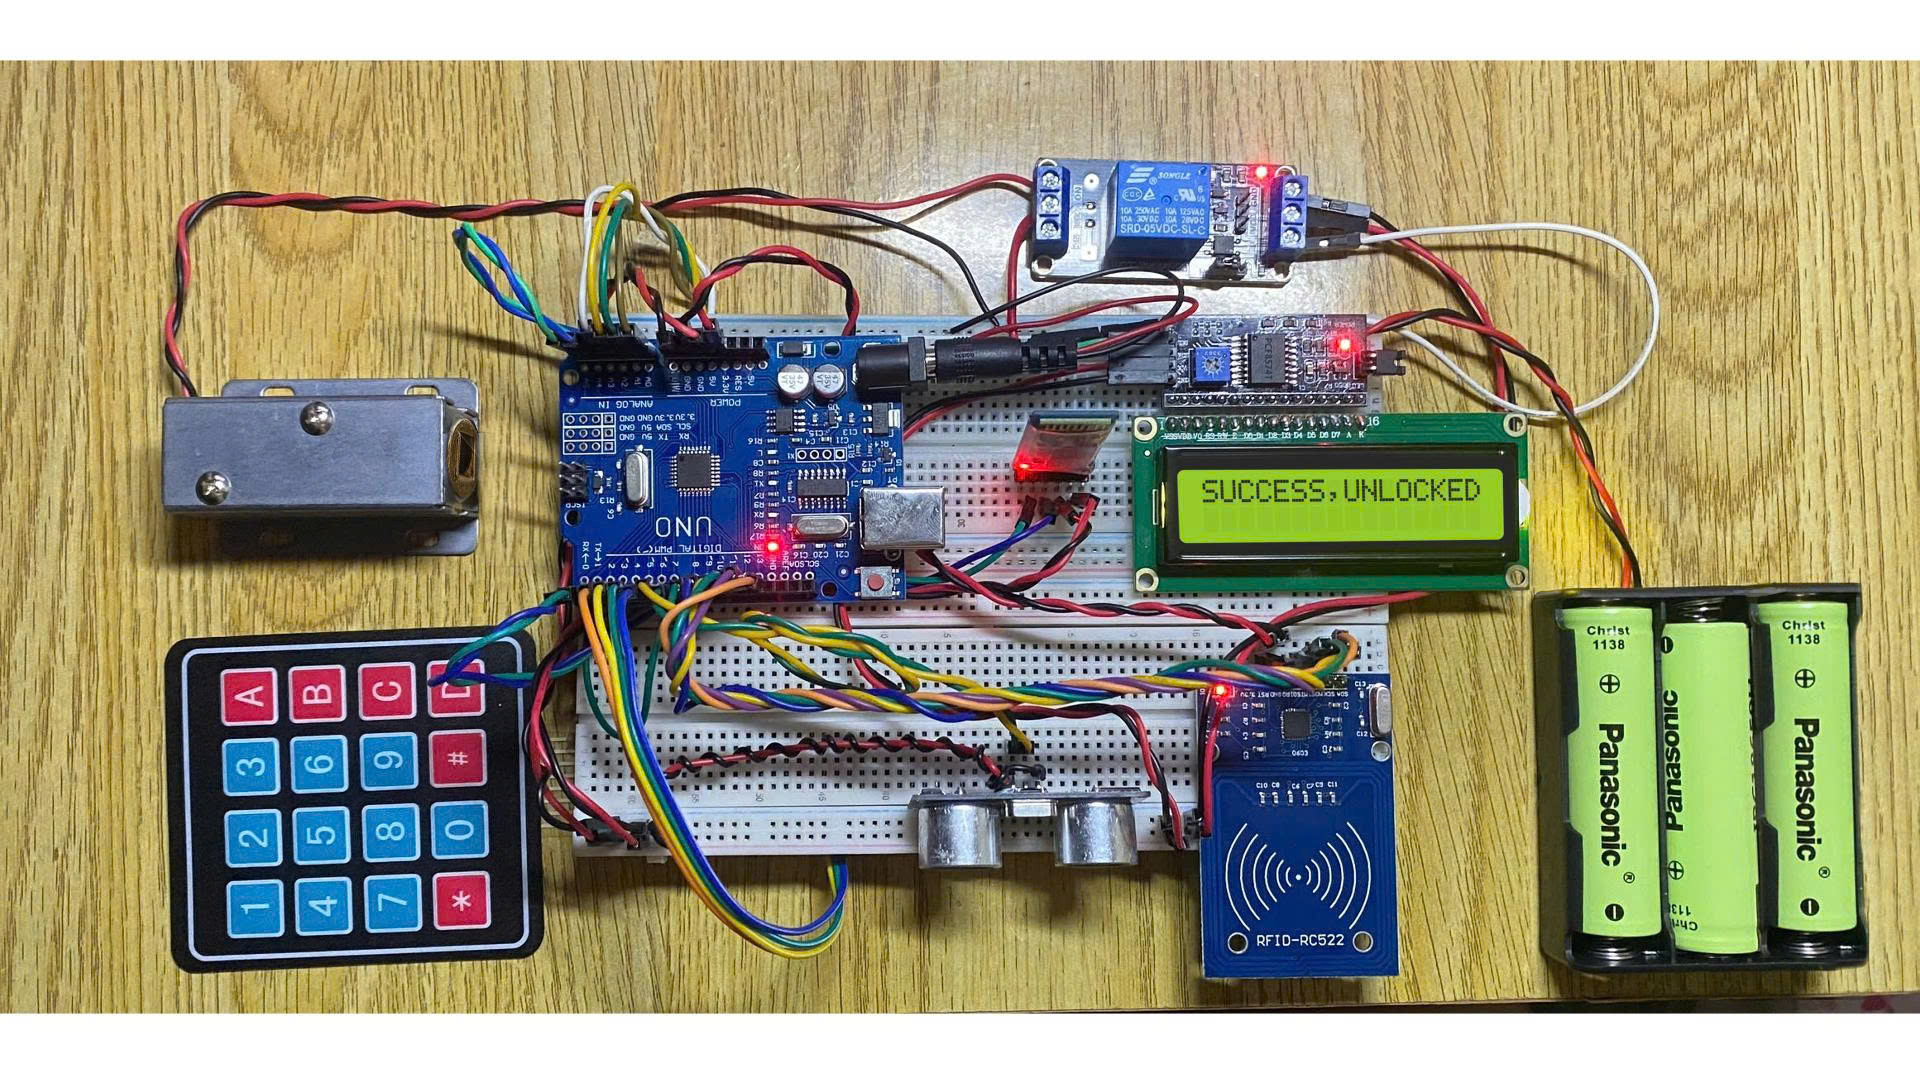
\includegraphics[width=0.75\textwidth]{mohinhsuse.jpg}
	\caption{Circuit UNLOODED Results.}
	\label{fig10}
\end{figure}	

User experience was also examined by inviting users to interact with the system using all three authentication methods. Most users adapted to the interface within two minutes. The LCD provided intuitive prompts such as “Enter Password,” “Access Granted,” or “Invalid Card,” which helped guide users through each step. Users appreciated the flexibility of choosing between keypad, RFID, or Bluetooth-based access.

Stress testing involved incorrect password entries, random RFID card scans, and simultaneous Bluetooth + keypad inputs. The system handled all exceptions gracefully, issuing retry prompts without freezing or crashing. Attempts to trigger relay operation manually or bypass authentication logic were effectively blocked by software safeguards. After power interruptions, the system resumed normal operation without requiring manual resets.

\begin{figure}[H]
	\centering
	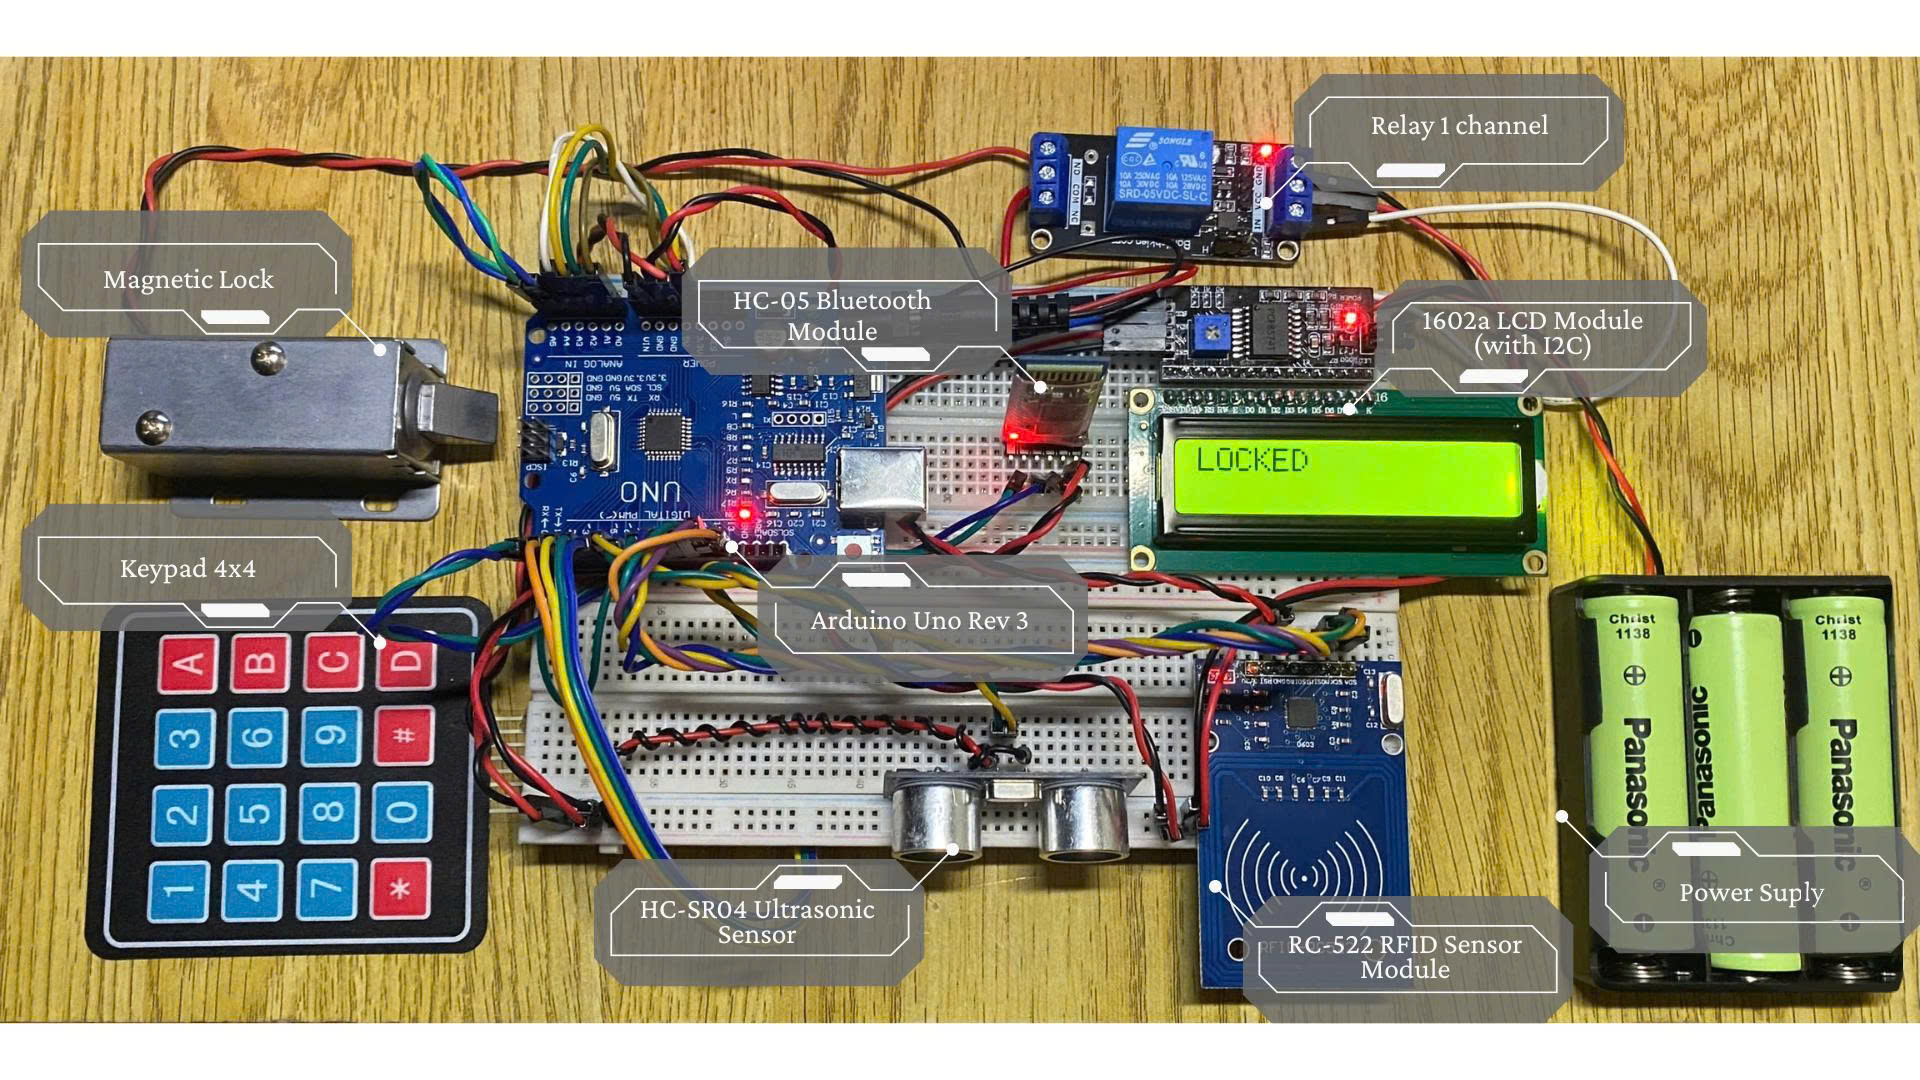
\includegraphics[width=0.75\textwidth]{mohinhdemo.jpg}
	\caption{Circuit LOODED Results.}
	\label{fig11}
\end{figure}	

\begin{figure}[H]
	\centering
	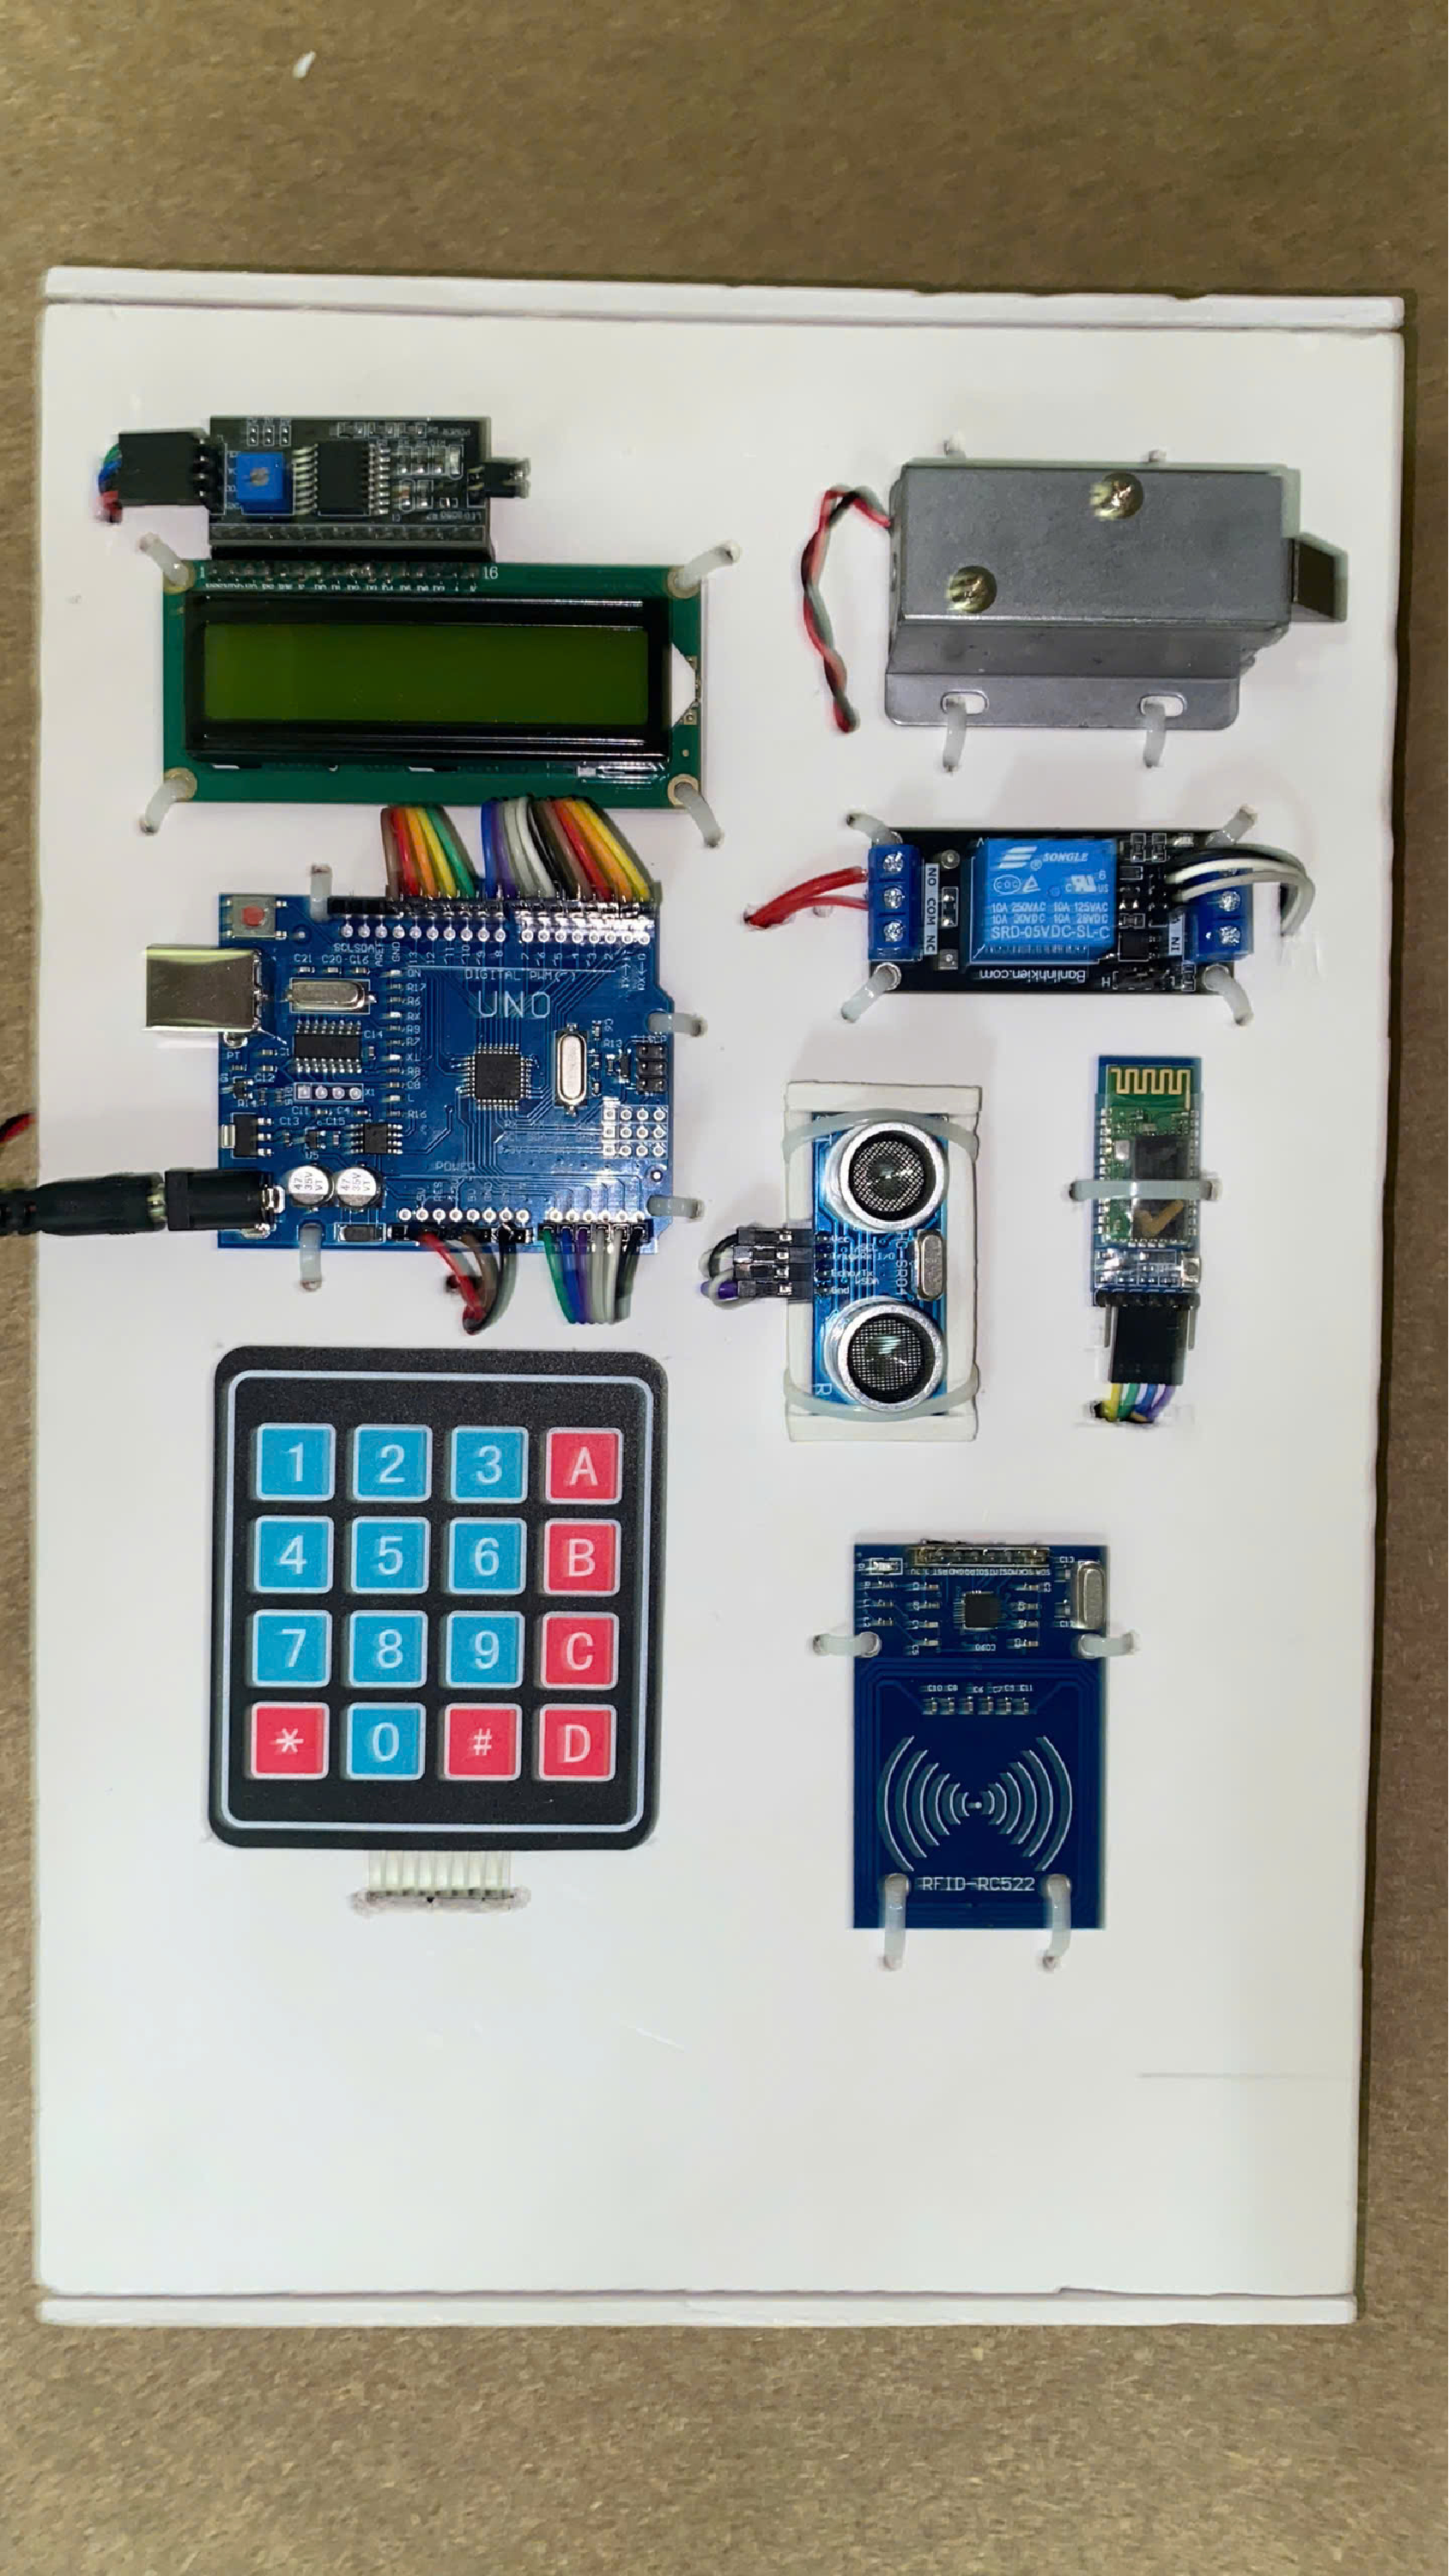
\includegraphics[width=0.3\textwidth]{FN.pdf}
	\caption{Circuit Smart Dook Results.}
	\label{fig12}
\end{figure}	

A summary of all module performance metrics is provided in Table II. All core modules achieved success rates of $96–100\%$, with fast response times and stable behavior. These experimental outcomes demonstrate that the smart door lock system operates effectively under real-world constraints, offering robust access control with responsive user interaction, low power consumption, and modular expandability. With its multi-authentication capabilities and integration of standard communication protocols, the system is well-suited for deployment in homes, labs, offices, and other access-restricted areas. Future improvements may include internet-based access control via Wi-Fi modules (e.g., ESP32), mobile app integration, or cloud logging for access history.

\renewcommand{\arraystretch}{1.3}  % giãn dòng bảng
  % Tăng khoảng cách dòng cho bảng

\begin{table}[H]
	\centering
	\caption{Summary of Experimental Performance}
	\begin{tabular}{|l|c|c|p{7cm}|}
		\hline
		\textbf{Module} & \textbf{Success Rate} & \textbf{Avg. Response Time} & \textbf{Notes} \\
		\hline
		Ultrasonic Sensor & 96\% & 0.6 s & Minor false positives due to environmental noise \\
		\hline
		Keypad Input & 100\% & 1.2 s & Includes password verification and debounce handling \\
		\hline
		RFID Reader & 100\% & 0.3 s & High reliability but limited to short-range tags \\
		\hline
		Bluetooth Module & 98\% & 1.5 s & Occasional delay during initial pairing with smartphone \\
		\hline
		Relay Control & 100\% & <0.1 s & Provides instant lock/unlock feedback \\
		\hline
		LCD Display & 100\% & -- & Displays clear and timely user messages \\
		\hline
		EEPROM Access & 100\% & <0.2 s & Fast read/write operations with stable performance \\
		\hline
		System Stability & 100\% & -- & Continuous operation without any crash or freeze \\
		\hline
	\end{tabular}
\end{table}

\subsection{Discussion}

This smart door lock system contributes to broader trends in smart living and sustainable development. As urban environments become more connected through the Internet of Things (IoT), smart security solutions are becoming foundational infrastructure for smart cities. The presented system fits naturally into this context. With its low energy consumption, ability to operate autonomously, and potential to be networked with other smart devices such as surveillance cameras, fire alarms, or smart lighting systems, it goes beyond being a stand-alone lock—it becomes a node in a smart ecosystem.
From the user perspective, the system emphasizes both security and convenience. The use of a multi-layered authentication process ensures that unauthorized access becomes significantly more difficult. Even if one method is compromised (e.g., someone knows the password), the other layers such as RFID verification or mobile approval act as safeguards. This layered approach reflects modern cybersecurity best practices adapted for physical environments. Furthermore, features like temporary unlocking via Bluetooth or automatic relocking help accommodate real-life situations, such as letting a family member or a delivery person in, without permanently compromising security.
In terms of technical scalability, the system is designed in a way that invites improvement. Developers could expand its features with minimal changes to the core design. For example, a buzzer could be added to alert owners of failed login attempts or tampering. A GSM module could be used to send SMS alerts in case of unauthorized access or power failure. Integration with a cloud-based database could allow remote management and access logs stored on the web, making it suitable for Airbnb hosts, rental properties, or office security. Furthermore, Wi-Fi support via modules like the ESP8266 could transform the system into a fully connected IoT device capable of being monitored and controlled from anywhere in the world.
Beyond its technical features, the project highlights the importance of user-centered design. The addition of an LCD display ensures clear feedback to the user, making the system intuitive even for non-technical users. Whether it's showing a welcome message, notifying a wrong password attempt, or confirming successful access, visual feedback enhances trust and ease of use. The ultrasonic sensor further demonstrates this philosophy by waking up the system only when needed, enhancing interactivity while conserving power.
From an educational and social impact perspective, the project showcases how low-cost, open-source hardware and software can be used to solve real-world problems. It encourages a do-it-yourself (DIY) mindset that empowers individuals and small communities to create custom solutions tailored to their needs, rather than relying solely on expensive commercial systems. This has special relevance in developing regions, where budget-friendly innovations can make a significant difference in security and daily living conditions.
Lastly, the system aligns well with current global security demands in both residential and industrial sectors. In places with high population density, shared entryways, or temporary accommodation settings, managing physical keys can be inefficient and risky. Smart locks like this one offer a digital alternative that is not only secure but also highly manageable. Changes in user access, such as removing or adding an RFID card, can be performed in seconds, without any need to change physical locks.
In conclusion, the smart door lock system presented here is a compelling prototype that balances affordability, security, expandability, and user-friendliness. Its practical applications extend from individual households to commercial properties and educational institutions. With minor enhancements, it could serve as a reliable and scalable security solution for the modern world. The project thus proves not only the feasibility of building such a system with accessible resources but also its readiness for real-life deployment in the growing landscape of smart infrastructure.

\section{Conclusion}
The smart door lock system offers a comprehensive and intelligent solution for modern access control, combining various authentication technologies to enhance both security and user convenience. By integrating ultrasonic distance sensing, RFID scanning, keypad PIN entry, and Bluetooth-based smartphone verification, the system ensures that only authorized users can gain entry. The Arduino Uno serves as the central controller, efficiently managing input signals, verifying credentials stored in EEPROM or flash memory, and activating output devices such as relays and electromagnetic locks based on authentication results. Notably, the design follows a power-efficient strategy by activating high-consumption modules like Bluetooth and the relay only when human presence is detected, thereby optimizing energy use—especially important for battery-powered or off-grid deployments. In addition to local control, the system supports remote access and status monitoring via Bluetooth, enhancing user interaction through a dedicated mobile application. It also offers administrative flexibility by allowing authorized users to update stored credentials, ensuring adaptability over time. With its modular structure, the system can be easily extended to include additional components like fingerprint scanners, camera modules, or cloud-based data logging, making it suitable for both residential and commercial applications. Overall, the project represents a scalable, secure, and IoT-ready smart lock architecture that meets the growing demand for intelligent home and office security systems.

\begin{thebibliography}{99}
	
	\bibitem{ref1}
	A. Singh and R. Kaur, ``Review of smart door locking system,'' \textit{International Journal of Engineering and Techniques (IJET)}, vol. 4, no. 3, pp. 107--110, 2018. [Online]. Available: \url{https://www.ijetjournal.org}
	
	\bibitem{ref2}
	T. M. Chen, ``Smart locks: Challenges and research opportunities,'' \textit{IEEE Consumer Electronics Magazine}, vol. 9, no. 2, pp. 18--21, Mar. 2020, doi: \href{https://doi.org/10.1109/MCE.2020.2966432}{10.1109/MCE.2020.2966432}
	
	\bibitem{ref3}
	M. Banzi and M. Shiloh, \textit{Getting Started with Arduino}, 3rd ed., Sebastopol, CA, USA: Maker Media, 2014.
	
	\bibitem{ref4}
	D. Kumar and A. Pandey, ``Multi-factor authentication using RFID and mobile devices,'' \textit{International Journal of Computer Applications}, vol. 169, no. 5, pp. 1--5, Jul. 2017.
	
	\bibitem{ref5}
	S. Rajalakshmi and G. Thilagavathi, ``IoT-based smart door lock system,'' in \textit{Proc. IEEE Int. Conf. on Smart Structures and Systems (ICSSS)}, Chennai, India, Mar. 2019, pp. 1--5, doi: \href{https://doi.org/10.1109/ICSSS.2019.8882827}{10.1109/ICSSS.2019.8882827}
	
\end{thebibliography}

\bibliographystyle{IEEEtran}
\end{document}